\documentclass[11pt,twoside]{extarticle}
\usepackage{floatrow}
\usepackage{etex}
\usepackage[english]{babel}
\usepackage{url}
\def\UrlBreaks{\do\/\do-}
\usepackage[breaklinks]{hyperref}
\usepackage{comment}

\usepackage[figuresright]{rotating}
\usepackage[margin=1.2in]{geometry}
\usepackage{setspace}
\renewcommand{\baselinestretch}{1.3}
\usepackage{booktabs, multicol}
\usepackage{threeparttable}
\usepackage{pdflscape}
\usepackage{xcolor}
\usepackage{amstext}
\usepackage{pgfplots}
\usepackage{color}
\usepackage{soul}
\usetikzlibrary{shapes,positioning,matrix,calc,shapes,shapes.multipart,shapes.misc,arrows,chains,fit,plotmarks}
\usetikzlibrary{decorations.text}

\usepackage{eurosym}
\usepackage{amssymb}
\usepackage{amsfonts}
\usepackage{afterpage}
\usepackage{epsfig}
\usepackage{upgreek}
\usepackage{commath}
\usepackage{enumitem}
\usepackage{subfigure}
\usepackage{indentfirst}
\usepackage{xr}
\usepackage{dsfont}
\usepackage{cleveref}
\usepackage{titlesec}
\usepackage{titling}
\usepackage{multibib}
\usepackage{makecell}
\usepackage{soul}
\usepackage{arydshln}
\usepackage{mathrsfs}
\usepackage{ragged2e}
\newcites{online}{References}
\allowdisplaybreaks

\usepackage[normalem]{ulem}

\setcounter{MaxMatrixCols}{10}

\newtheorem{theorem}{Theorem}
\newtheorem{acknowledgement}{Acknowledgement}
\newtheorem{algorithm}{Algorithm}
\newtheorem{assumption}{Assumption}
\newtheorem{axiom}{Axiom}
\newtheorem{case}{Case}
\newtheorem{claim}{Claim}
\newtheorem{conclusion}{Conclusion}
\newtheorem{condition}{Condition}
\newtheorem{conjecture}{Conjecture}
\newtheorem{corollary}{Corollary}
\newtheorem{criterion}{Criterion}
\newtheorem{definition}{Definition}
\newtheorem{example}{Example}
\newtheorem{observation}{Observation}
\newtheorem{exercise}{Exercise}
\newtheorem{fact}{Fact}
\newtheorem{lemma}{Lemma}
\newtheorem{notation}{Notation}
\newtheorem{problem}{Problem}
\newtheorem{proposition}{Proposition}
\newtheorem{remark}{Remark}
\newtheorem{solution}{Solution}
\newtheorem{summary}{Summary}
\providecommand*{\theoremautorefname}{Theorem}
\providecommand*{\factautorefname}{Fact}
\providecommand*{\lemmaautorefname}{Lemma}
\providecommand*{\propositionautorefname}{Proposition}
\providecommand*{\corollaryautorefname}{Corollary}
\providecommand*{\definitionautorefname}{Definition}
\providecommand*{\remarkautorefname}{Remark}
\providecommand*{\subfigureautorefname}{Subfigure}
\providecommand*{\algorithmautorefname}{Algorithm}
\providecommand*{\assumptionautorefname}{Assumption}
% Capitalise section/subsection so \autoref{sec:X} prints "Section X" not "section X".
% Deferred to \AtBeginDocument because hyperref defines these names late.
\AtBeginDocument{%
  \renewcommand*{\sectionautorefname}{Section}%
  \renewcommand*{\subsectionautorefname}{Section}%
}
\newenvironment{proof}[1][Proof]{\noindent \textbf{#1.} }{\ \rule{0.5em}{0.5em}}
\geometry{left=1.2in,right=1.2in,top=1.3in,bottom=1.3in}
\renewcommand{\baselinestretch}{1.3}
\newcommand{\newln}{\\&\quad\quad{}}
\newcommand{\parenthnewln}{\right.\\&\left.\quad\quad{}}
\usepackage{bbm}

\usepackage{longtable}
\usepackage[para]{threeparttablex}

\usepackage{float}
\usepackage[titletoc,title]{appendix}
\raggedbottom

\usepackage{amsmath}
\usepackage{bm}
\usepackage{lineno}

\usepackage[T1]{fontenc}
\usepackage{palatino}

\usepackage{graphicx}

\hypersetup{
   colorlinks=true,linkcolor=blue,citecolor=blue, filecolor=magenta, citebordercolor=yellow,
   linkbordercolor = magenta
}

\usepackage{graphicx}
\graphicspath{{../output/figures/}{../../output/figures/}}
\usepackage{subfigure}
\floatsetup[figure]{font=footnotesize}

\floatsetup[table]{capposition=top}
\floatsetup[table]{font=footnotesize}

\floatsetup{style=plain,footposition=bottom}
\floatsetup[figure]{capposition=bottom}

\usepackage{multirow}
\newcommand{\specialcell}[2][c]{%
        \begin{tabular}[#1]{@{}c@{}}#2\end{tabular}}

\makeatletter
\renewcommand\@makefntext[1]{%
    \parindent 1em%
    \@thefnmark.~#1$\qquad$}
\makeatother

\usepackage{tabularx}
\newcolumntype{R}{>{\raggedleft\arraybackslash}X}
\newcolumntype{L}{>{\raggedright\arraybackslash}X}
\newcolumntype{C}{>{\centering\arraybackslash}X}

\usepackage[figuresright]{rotating}

\usepackage[font=normalsize,format=plain,labelfont=bf,up,textfont=up,justification=centering]{caption}
\captionsetup[table]{labelsep=space}
\captionsetup[figure]{labelsep=space}
\addto\captionsenglish{%
\renewcommand{\figurename}{FIGURE}
\renewcommand{\tablename}{TABLE}}
\renewcommand{\thesubfigure}{(\Alph{subfigure})}

\usepackage{natbib}
\newcommand{\cites}[1]{\citeauthor{#1}'s (\citeyear{#1})}

\usepackage{pdflscape}

\usepackage[titletoc]{appendix}
\usepackage{titletoc}

% Resolve \input paths relative to the .tex file rather than pdflatex's cwd,
% so the file compiles whether you build from model/ or from this submission folder.
\usepackage{import}

\title{Manufacturing Enemies in Political Contests}
\author{Haotian (George) Bai}
\date{\today}

% Styled cross-document reference to the separate supplementary PDF.
% Cross-PDF clicks do not work, so this renders as plain text in the
% hyperref linkcolor (blue) to match other reference styling.
\newcommand{\suppmat}{\textcolor{blue}{Supplementary Materials}}

\begin{document}

\maketitle

\begin{abstract}
What is the purpose of identity-coded policies (symbolic policies) targeted at domestic minorities? 
With each group's effort determined by collective mobilisation, the majority and minority contest over security in identity.
Social conflict is determined by aggregated effort.
Two parties (\emph{Hawk} and \emph{Dove}) compete in elections with probabilistic retrospective voting.
Symbolic policy allows the \emph{Hawk} party to manufacture a threat that reduces majority free-riding.
This makes its advantage in identity security electorally salient, and therefore substitutes identity politics for economic competence.
%I study political contest of two parties (with different contest technology) where symbolic policies are within the strategy set of each party.
%Individual choose their level of identity-related mobilisation subjected to a collective action problem, and then vote myopically.
A two-period model shows that Hawk's vote share is non-monotonic in the grievance it manufactures.
Once the Hawk generate sufficient minority mobilisation, future conflict continues despite incumbent policies.
%Baseline analysis shows symbolic policy allows a security-advantaged party to manufacture a visible threat that relaxes majority free-riding, makes its coercive-capacity advantage electorally salient, and substitutes identity salience for economic competence. 
%However, Hawk's vote share is non-monotonic in the grievance it manufactures. 
I further study the long-run equilibria under symbolic policies by iterating the process into infinite periods.
With sufficiently high voter's weight on identity security, perturbed Markov chain characterises two regimes (a \emph{Hawk}-trap or recurrent \emph{Hawk}-\emph{Dove} cycles). 
The equilibrim is determined by the depreciation rate of monority mobilisation.
The predictions match empirical patterns in India's cattle-slaughter ban, among other cases.
Finally, I discuss why banning symbolic policies may backfire.\\

\emph{JEL Codes: D72, D74, P16, Z18}.

\end{abstract}

\begin{center}
\small\textit{Total word count: 19190.}
\end{center}

\clearpage

\begin{quote}
\textit{``Only one thing is worse than communal war --- and that is when your government exploits communal differences, stokes ethnic and religious fears, all in the pursuit of power.''}

\hfill --- A. Sivanandan, \textit{``Ethnic Cleansing in Sri Lanka''}
\end{quote}

\section{Introduction}

% Paragraph 1 — Opening: the phenomenon

There has been a widespread rise in identity-coded policies (symbolic policies) targeting domestic minority groups in electoral democracies. By symbolic policies, I mean deliberate control over cultural, religious, and ethnic identities on minority groups. These policies include restrictions on diet, dress, marriage, or language regulations, chosen by an elected majority party and directed at a visible domestic out-group. In the last decade, legislative waves in major Indian states have criminalised cow-slaughtering with penalties of up to ten years' imprisonment. Between 2012-2018, over forty cow-related deaths were documented, whose victims were mostly Muslim.\footnote{\href{https://www.hrw.org/report/2019/02/19/violent-cow-protection-india/vigilante-groups-attack-minorities}{Human Rights Watch (2019): Violent Cow Protection in India Vigilante Groups Attack minorities}, last access Apr $17^{th}$, 2026.} \autoref{fig:policy_cumulative_rollout} documents the rollout of cow-slaughter bans. The pattern has been repeated across electoral democracies, from the post-2016 anti-immigration turn in the United States, to the Uribista policies under Álvaro Uribe Vélez. Such polices are also seen in non-democracies with political competition.\footnote{Iranian principalists deploy hijab enforcement and morality-policing campaigns to combat economics reformists when they gain popularity \citep*{bajoghliIranReframedAnxieties2020}. Chinese Communist Party (CCP) has divergent policies on ethnic groups as Politburo faction shifts \citep*{leiboldEthnicPolicyChina2013}. \citet*{francoisFactionsNondemocraciesTheory2023} introduces CCP factions, policies, and welfare in China. \citet*{francoisHowPowerShared2015} documents ethnic-political contests in Africa.} These features also do not appear in economic theories of political accountability in political contests, which ignore identity considerations. Why does a rising number of political groups obtain and sustain power by targetting a non-pivotal minority group?

% \citep*{barroControlPoliticiansEconomic1973,ferejohnIncumbentPerformanceElectoral1986}

% --- Figure inlined right after paragraph 1 of Introduction -----------------
% Moved out of the trailing Figures section per supervisor request: figures
% should appear within the text where they are first discussed. The opening
% paragraph references this figure in its footnote, so the rollout pattern
% should be visible to the reader as they finish paragraph 1.
\begin{figure}[!h]
    \centering
    
\includegraphics[width=0.92\textwidth]{policy_cumulative_rollout.jpg}
    \caption{\normalsize\bf Cumulative Cattle-Slaughter Ban Rollout, 1950--2020.}
    \label{Figure:policy_cumulative_rollout}\label{fig:policy_cumulative_rollout}
    \floatfoot*{\footnotesize\textit{Notes}: Cumulative count of state-years of cattle-slaughter bans across six different categories. The $2015$--$2017$ acceleration coincides with the first Modi-government term. Construction of the policy panel is in the \suppmat.}
\end{figure}
% ----------------------------------------------------------------------------

% Paragraph 2 — Consequently: policy and scholarly interest, and the gap
In 2019, India's Citizenship Amendment Act ignited the largest sustained urban protest since independence \citep{jaffrelotModisIndiaHindu2021}.\footnote{The \emph{Woman, Life, Freedom} protests in Iran after the 2022 death of Mahsa Amini and the wide-spread anti-immigrants Republican campaigns before the 2024 United States presidential election show similar patterns.} However, it is not clear why is so much policy attention directed toward non-pivotal minoirty groups. Why should the majority treat identity-related behaviours (e.g., dress and food) of such an outgroup as a major threat? Political economists have also not fully understood why majority parties choose such policies in the first place, why voters reward them, and why the same mechanism produces durable one-party dominance in some polities and recurrent turnovers in others.

% Paragraph 3 — Placing the paper, stating the aim, and the toolkit

This article introduces the manufacturing of enemies in political contests to the economics of identity and electoral competition \citep*{shayoModelSocialIdentity2009,glaeserPoliticalEconomyHatred2005,gennaioliIdentityPolitics2023}.\footnote{A large literature has captured electoral mobilisation of communal violence by majority parties in divided democracies.} My aim is to explain why elected majority parties choose symbolic policies against domestic minorities, and to characterise the long-run consequences of doing so for political competition and social conflict. In attempting to do so, I draw on developments in contest theory and the political economy of electoral accountability.

% Paragraph 4 — The model

In my model, symbolic policy initiates a two-sided contest over public security (in identity) between a majority group and a domestic minority. 
Following \citet*{baligaStrategyManipulatingConflict2012}, two parties compete for cotes, one with a comparative advantage in delivering economic public goods (e.g.\ the BJP), the other in coercive and organisational capacity (eg.,\ the Congress). 
The minority includes agents sensitive to their minority identities (e.g.\ Muslim). They mobilise to preserve their identity, through protest or voilence. 
The majority internalize monority's mobilisation and conduct their own collective actions in preserving identity, with their own protest or voilence actions.
I model social conflict as the sum of voilence from two sides.
Subject to the free-riding problem, mobilisation (both the majority and minority groups) only occurs when grievance among their members is large enough.
The electoral return to symbolic policy is therefore highest when the security-oriented party (\emph{Hawk}) has an organisational advantage that only arises under conditions of social conflict, or when the economic potential of its opponent (\emph{Dove}) is sufficiently large that it cannot be offset on the consumption dimension alone.

% Paragraph 5 — Linking the model to observed patterns

%This enables me to link the manufacturing of enemies to the economic and political transformations that have accompanied recent electoral democracies. The most important changes were the rise of redistributive politics after the Cold War, the widening of the electoral franchise through liberalising the minority in post-colonial areas, and the emergence of parties whose organisational base lies in religious, paramilitary, or coercive associations. 
I show manufacturing enemies comes at the cost of economic and social disruption by making the security dimension of contest electorally. I aim to develop a unified framework for understanding the contemporary use of symbolic policy in otherwise disparate settings: India's cow-slaughter bans under the BJP \citep{jaffrelotModisIndiaHindu2021}, the Republican Party's post-2016 transformation to immigration and domestic-security framing in the United States \citep{sidesIdentityCrisis20162019,mutzStatusThreatNot2018}, the morality-police enforcement in Iran \citep{bajoghliIranReframedAnxieties2020}, and the Uribismo in Colombia \citep*{acemogluMonopolyViolenceEvidence2013}. It suggests one explanation for the important role that security-coded mobilisation plays during periods of economic liberalisation, when the non-hawkish coalition's comparative advantage in economic delivery is at its greatest. It also helps us to understand the strategies of political groups organized with religious, paramilitary, or coercive associations after the Cold War, especially in the post-colonial world.

% Paragraph 6 — key strategies 

I deliver three key insights on the strategy of manufacturing enemies. First, the Hawk's electoral return to symbolic policy is \emph{non-linear} in minority's mobilisation. Above certain threshold determined by both party's technology, further provocation decreases the security premium it was deployed to manufacture. Second, the slow-decaying property of minority mobilisation generates the \emph{paradox of restraint}. A Hawk who has accumulated enough inherited mobilisation optimally legislates no symbolic policy. Third, the \emph{paradox of competence}. Conditional on Hawk incumbency, more realised disorder during its tenure predicts higher re-election probability, since the inherited mobilisation makes the Hawk's coercive advantage indispensable to voters.

% I formalise this mechanism in a two-sided Tullock contest with within-group collective action, embedded in a probabilistic-voting game with retrospective accountability. The polity is partitioned into a majority, represented in the electoral arena by two parties and a non-voting minority. The two parties differ along two technological dimensions: the Hawk has higher coercive capacity but lower public-goods capacity. In each period the incumbent commits to a symbolic-policy intensity; conditional on $d$, the majority and minority each choose mobilisation effort subject to a private quadratic cost, and the within-period contest produces a closed-form equilibrium dominance probability for each party. The minority's effective stake decays at $\rho$. The voter is \emph{myopic-retrospective}: she observes the realised state, computes each candidate's stationary per-period welfare under its best-reply at that state, and votes for whichever delivers more by weighting the Hawk's security advantage against the Dove's economic advantage and the real economic destruction symbolic policy imposes. My baseline analysis sloves a two-period game with. The period-1 Hawk anticipates how its period-1 policy shapes the inherited mobilisation that the period-2 voter then evaluates against the period-2 incumbent's stationary best-reply. I discuss assumptions in \autoref{sec:model_v3}.

% Paragraph 7 — Long-run extension

To study the long-run consequences of manufactured enemies, I iterate the same within-cycle game under the same myopic-retrospective voting rule, perturbed by an i.i.d. salience shocks. The state, characterised by minority mobilisation and incumbency status, then evolves as a perturbed Markov chain whose long-run regime is determined by a single primitive: the depreciation rate $\rho$ of the mobilisation stock. When $\rho$ is small the deterministic basin around the Hawk attractor is deep, voter-decisive shocks are absorbed, and the system locks into a stochastically forward-invariant \emph{conflict trap}. When $\rho$ is large the same shocks drive ergodic Hawk--Dove \emph{cycles} in which a more successful Hawk paradoxically becomes more likely to lose office. The two long-run regimes therefore emerge as parameter regions of a single perturbed chain, with $\rho$ playing the role of an effective noise scale \citep*{youngEvolutionConventions1993,youngIndividualStrategySocial1998a}. 

% Paragraph 8 — Ethnic Contest

Let me turn to the relationship to and departures from existing work. This paper first contributes to the theoretical literature on the economics of intergroup conflict and contest design.
The canonical formal approach models intergroup conflict as a contest where the salient cleavage (class, religion, or ethnic identities) and the intensity of social conflict are determined by exogenous parameters such as group size, group budget, within-group inequality, or shocks on economic capacity \citep*{estebanConflictDistribution1999, estebanSalienceEthnicConflict2008, caselliTheoryEthnicConflict2006, acharyaElectoralCampaignsDynamic2024}.\footnote{Empirical literature corresponds to these theoretical advances \citep{dalbóWORKERSWARRIORSCRIMINALS2011, rohnerWarSignalsTheory2013, dubeCommodityPriceShocks2013}.} 
A large literature also formalises how incumbents initiate conflict to divert attention from economic underperformance \citep*{hessWarDemocracy2001}. 
However, the contest environment itself remains isolated from the political process. 
My theoretical departure is to combine political competition and social conflict by embedding a two-sided Tullock contest with endogenous collective action into a political agency framework.
Unlike a standard neutral principal optimising rules to maximise joint effort \citep*{skaperdasContestSuccessFunctions1996,jiaStochasticDerivationRatio2008,barutSymmetricMultiplePrize1998,fangTurningHeatDiscouraging2020}, the political principal (i.e.\ the party) is biased in my model. 
I formalise a novel mechanism of conflict as an endogenous electoral instrument \citep{iyerReligiousRiotsElectoral2018, mitraImplicationsEconomicTheory2014}.

% Paragraph 9 — Identity Politics

Second, I advance the formal literature on the political economy of identity and issue salience. 
Existing theories model the political usage of identity either as a demand-side expressive distortion of standard redistributive preferences \citep{shayoModelSocialIdentity2009, besleyRiseIdentityPolitics2019, gennaioliIdentityPolitics2023}, or as a supply-side informational problem where elites manipulate beliefs or supply hatred to split voter coalitions \citep*{glaeserPoliticalEconomyHatred2005, baligaStrategyManipulatingConflict2012, izzoIdeologicalCompetition2023, callanderCauseEffectPolitical2022}. 
Recent models also show how elites strategically substitute identity cleavages for economic redistribution to maintain power \citep*{acemogluKleptocracyDivideandRuleModel2004,padróimiquelControlPoliticiansDivided2007,mukandPoliticalEconomyLiberal2020}. 
Classic divide-and-rule mechanisms typically rely on elite coordination failure or cheap-talk manipulation. 
By contrast, my mechanism does not rely on behavioural biases, asymmetric information about the state of the world, or cheap-talk coordination. 
Symbolic policies act as a technology that shifts the constraints of a collective-action subgame. 
The incumbent alters the policy space by forcing voters into a second-best environment in which coercive capacity becomes an unavoidable necessity. 
This provides a micro-foundation for the \emph{politics of fear} through endogenous threat.

% Paragraph 10 — Conflict as Electoral Strategy

Finally, my long-run extension contributes to the political-agency theory of electoral accountability.
Canonical retrospective-voting models \citep*{barroControlPoliticiansEconomic1973,ferejohnIncumbentPerformanceElectoral1986} have been extended to capture information design \citep*{banksRepeatedElectionsModel1993,przeworskiDemocracyAccountabilityRepresentation1999,sandroniWhenConfrontRole2018a,acharyaPoliticalAccountabilityMoral2025} and behavioural responses \citep*{levyCorrelationNeglectVoting2015,ortolevaOverconfidencePoliticalBehavior2015,liElectoralAccountabilitySelection2023,vaethVoterLearningUnidimensional2023}. 
A first strand of this literature embeds a slow-moving state variable (eg., accumulated reputation, persistent policy choices, or partisan beliefs) into an agency model and shows that this state generates hysteresis in retention thresholds and a continuation-value wedge between competing regimes \citep*{coatePolicyPersistence1999,padróimiquelControlPoliticiansDivided2007}. 
A second strand uses stochastic-stability tools to determine among multiple deterministic equilibria of a perturbed dynamic system via the invariant distribution of the perturbed Markov chain and the depth of each basin of attraction \citep*{kandoriLearningMutationLong1993a,meynMarkovChainsStochastic2012}. 
In my model, the inherited mobilisation stock plays the role of the persistent state variable inside the swing-voter rule, and the long-run regime is selected by the deterministic basin around the Hawk attractor in the perturbed chain. The regime-selecting parameter is the empirically identifiable depreciation rate of communal grievance.

% Paragraph 11 — Paper structure

The remainder of the paper proceeds as follows. \autoref{sec:empirical_facts} documents the four empirical facts of India's symbolic policy. \autoref{sec:model_v3} sets up the model and discusses key assumptions. \autoref{sec:block1} characterises the within-period contest technology. \autoref{sec:block2} solves the period-2 election. \autoref{sec:block3} steps back to the period-1 provocation problem and solves optimal electoral strategy under symbolic policies. \autoref{sec:dynamics_v3} embeds the same primitives in a perturbed Markov chain and shows possibilities of two long-run regimes. \autoref{sec:conclusion_v3} concludes.

%===================================================================================
% Empirical facts (tightened; see appendix for methodological detail)
%===================================================================================

\section{Empirical Motivation} \label{sec:empirical_facts}

I document four empirical facts about one of the most prominent symbolic policies in contemporary India, the cattle-slaughter ban.\footnote{Data sources are summarised in the \suppmat.} I ask when the legislative wave broke and how it spread, which party benefited electorally and on how, where in the federation the pattern took hold spatially, and what consequences it left for the targeted communities. I move beyond India and discuss three other cases of symbolic politics.

\begin{fact}\label{fact:1}
Symbolic legislation in India is accompanied by a rise in identity-related narratives on both the majority mobilisation and the minority counter-mobilisation.
\end{fact}

There have been no national-level prohibition on cow in India. 
For four post-independence decades, beef regulation remains a state-level matter, where enforcement is stricter in Jan Sangh or BJP-goverened states \citep*{jaffrelotHinduNationalistMovement1999}. 
The formal landscape on beef issues changed significantly after the 2014 victory of BJP. As in \autoref{fig:policy_cumulative_rollout}, there has been a sharp rise of related policies across states post 2014, after which a consecutive wave of legislation has extended bans from cows to other Bovine family, lowered the bar to proof guilty in slaughtering, and raised the maximum penalties of related behaviours.\footnote{Policy timing table is in the \suppmat. Maharashtra Animal Preservation (Amendment) Act 2015 and Haryana Gauvansh Sanrakshan Act 2015 are the typical cases. Similars amendment laws were followed by Gujarat, Jharkhand, Uttar Pradesh, Madhya Pradesh, and Uttarakhand.} 
To see who are the main advocates of such policy, I utilize a wide range of micro-survey data in India. I report my results in \autoref{fig:policy_and_identity}, in which I use household-level serveys (India Human Development Survey). The figures show support for cow-slaghter bans, support for the BJP, and Hindu religiousity are tightly correlated at the individual level. Hindu respondents support a ban at $89\%$ versus $51\%$ for non-Hindu respondents, and ban-supporting households are more likely to support the BJP. \footnote{Data construction available in related figurenotes.}

% --- Figure fig:policy_and_identity inlined here ----------------------------------
% Moved out of the trailing Figures section per supervisor request.
\begin{figure}[!h]
    \centering
    \subfigure[\bf Support cow-slaughter ban.]{\includegraphics[width=0.32\textwidth]{rpb_support_ban.jpg}}
    \subfigure[\bf Religious reason: support.]{\includegraphics[width=0.32\textwidth]{rpb_religious_pro.jpg}}
    \subfigure[\bf Religious reason: against.]{\includegraphics[width=0.32\textwidth]{rpb_religious_anti.jpg}}\\
    \subfigure[\bf Support BJP.]{\includegraphics[width=0.32\textwidth]{rpb_support_bjp.jpg}}
    \subfigure[\bf Oppose BJP.]{\includegraphics[width=0.32\textwidth]{rpb_against_bjp.jpg}}
    \caption{\normalsize\bf Religious Identity, Cattle-Ban Support, and BJP
    Alignment in IHDS-II Households.}
    \label{Figure:policy_and_identity}\label{fig:policy_and_identity}
    \floatfoot*{\footnotesize\textit{Notes}: Mean proportions with $95\%$
    confidence intervals from IHDS-II. Panels (a)--(c) split households by
    religion (Hindu vs.~non-Hindu) on (a) support for a cow-slaughter ban,
    (b) citing a religious reason for supporting the ban, and (c) citing a
    religious reason against the ban. Panels (d) and (e) split households
    by stated ban stance on (d) BJP support and (e) BJP opposition. Hindu
    and pro-ban households cluster on the BJP-support side; non-Hindu and
    anti-ban households cluster against. The household-level alignment in
    (a)--(e) and the legislative-rollout series in
    \autoref{fig:policy_cumulative_rollout} move together: states
    accelerate ban adoption exactly as the underlying identity-coded
    voter base over which the bans are politically salient is largest.
    Sample sizes and variable mappings in
    the \suppmat.}
\end{figure}
% ----------------------------------------------------------------------


%Independent India inherited a constitutional encouragement of cow protection (Article~48) but no national prohibition. For four post-independence decades beef regulation was a state-level matter, with stricter enforcement in a handful of Jan~Sangh- or BJP-governed states \citep*{jaffrelotHinduNationalistMovement1999}. The legal landscape changed discontinuously after the BJP's 2014 national victory: between 2015 and 2017 a wave of state-level legislation extended bans from cows to the entire bovine family, reversed the burden of proof, and raised maximum penalties to ten years' imprisonment. \autoref{fig:policy_cumulative_rollout} plots the cumulative count of state-years under each of the six cattle-slaughter bans and makes the post-2014 discontinuity visible at a glance.\footnote{Maharashtra Animal Preservation (Amendment) Act 2015 and Haryana Gauvansh Sanrakshan Act 2015 are the benchmark cases; analogous amendments followed in Gujarat, Jharkhand, Uttar Pradesh, Madhya Pradesh, and Uttarakhand. Construction details and a state-by-state timing table are in the \suppmat.} The household-level correlate is visible in the India Human Development Survey: support for cow-slaughter bans, support for the BJP, and Hindu religious identity are tightly linked at the individual level, as the five within-IHDS-II panels of \autoref{fig:policy_and_identity} show. Hindu respondents support a ban at $89\%$ versus $51\%$ for non-Hindu respondents, and ban-supporting households are markedly more likely to back the BJP.

Do these symbolic policies trigger parallel rise in narratives on identities? Do these policies mobilise minority muslim groups in India? To measure narratives, I turn to $3{,}328$ BJP-leadership texts from the party's official speech archive, the Prime Minister's Office, and BJP Lok~Sabha floor speeches (1996--2025). 
Also, for the Muslim side, I collect $3{,}792$-item proxy corpus of Muslim-voice news from Google-News-RSS harvest (2010--2025) and AIMIM Lok~Sabha speeches.\footnote{Speakers, queries, the keyword and Claude Haiku~4.5 classification prompt engineering workflow are reported in the \suppmat, where I also document the symmetric sampling process.} I report the result in \autoref{fig:narrative_timeseries}, which shows the monthly identity-coded share on the majority side and the counter-mobilisation share on the minority side.
The largest joint spike occurs along with 2019--20 Citizenship Amendment Act episode and the Shaheen~Bagh protests. During these periods, the majority identity content rises from near $5\%$ to above $30\%$ and minority counter-mobilisation from near zero to above $70\%$. 
Furthermore, majority identity content leads minority counter-mobilisation by roughly three months ($r=0.55$ at the peak cross-correlation), with less obvious secondary spikes.\footnote{Near the 2022 hijab cycle and the 2024 Waqf Bill.}

% --- Figure fig:narrative_timeseries inlined here ----------------------------------
% Moved out of the trailing Figures section per supervisor request.
\begin{figure}[!h]
    \centering
    \subfigure[\bf Original pair: BJP speeches vs Muslim-voice news (asymmetric, Haiku~4.5).]{%
        \includegraphics[width=0.82\textwidth]{narrative_timeseries.jpg}%
        \label{fig:narrative_timeseries_original}%
    }\\
    \subfigure[\bf Balanced pair: BJP news vs Muslim-voice news, identity~$+$~action (symmetric).]{%
        \includegraphics[width=0.82\textwidth]{narrative_timeseries_balanced.jpg}%
        \label{fig:narrative_timeseries_balanced}%
    }
    \caption{\normalsize\bf Majority and Minority Identity-Coded Narrative
    Share, India 2018--2025.}
    \label{Figure:narrative_timeseries}\label{fig:narrative_timeseries}
    \floatfoot*{\scriptsize\textit{Notes}: Both panels report the monthly
    share of identity-coded content (majority, red) and counter-mobilisation
    content (minority, blue), six-month centred rolling means; numerators
    are divided by total monthly content in their own corpus.
    \textbf{Panel~(A)}: original asymmetric pair. Majority $N=3{,}328$
    direct speeches from \texttt{bjp.org/speeches}, \texttt{pmindia.gov.in},
    and BJP~Lok~Sabha; minority $N=3{,}792$ news-outlet items from a
    $65$-query Google-News harvest plus nine AIMIM~speeches; both classified
    by Claude~Haiku~4.5. Medium is asymmetric (speeches vs news), so
    levels are not directly comparable. \textbf{Panel~(B)}: balanced
    symmetric pair. A parallel BJP-news corpus ($N=5{,}811$) is harvested
    via the same Google-News~RSS pipeline against the same outlet set; the
    minority corpus is re-classified with the same keyword scheme. Each
    series plots a strictly symmetric (identity~$+$~action) flag, requiring
    both an identity keyword and an action verb (assertive on the majority
    side: rally, march, gather, organise, defend, vow, lead, etc.; reactive
    on the minority side: protest, dharna, satyagraha, oppose, agitation,
    bandh, etc.), so background identity mentions cannot inflate either
    series. Vertical dashed lines mark the December~$2019$ CAA passage,
    January~$2024$ Ram-Mandir consecration, and August~$2024$ Waqf
    Amendment Bill. Construction details, full lexicons, and category
    definitions in the \suppmat.}
\end{figure}
% ----------------------------------------------------------------------


%The legislative wave was accompanied by a parallel rise in identity-coded rhetoric on both sides. I assemble $3{,}328$ BJP-leadership texts from the party's official speech archive, the Prime Minister's Office, and BJP Lok~Sabha floor speeches (1996--2025), and a $3{,}792$-item proxy corpus of Muslim-voice news from a $65$-query Google-News-RSS harvest (2010--2025) supplemented by AIMIM Lok~Sabha speeches.\footnote{Speakers, queries, the keyword and Haiku~4.5 classification protocols, the asymmetry between primary-source archives, and a balanced symmetric BJP-news robustness corpus are reported in the \suppmat.} \autoref{fig:narrative_timeseries} plots the monthly identity-coded share on the majority side and the counter-mobilisation share on the minority side. The 2019--20 Citizenship Amendment Act episode and the Shaheen~Bagh protests are the largest joint spike: majority identity content rises from near $5\%$ to above $30\%$ and minority counter-mobilisation from near zero to above $70\%$. Majority identity content leads minority counter-mobilisation by roughly three months ($r=0.55$ at the peak cross-correlation), with smaller secondary spikes at the 2022 hijab cycle and the 2024 Waqf Bill.

\begin{fact}\label{fact:2}
In India, some states show long uninterrupted BJP spells and others show alternation between BJP and INC (Indian National Congress). Conditional on BJP incumbency, the probability of re-election rises with the realised Hindu--Muslim conflict over the prior tenure.
 
%Long uninterrupted BJP spells (e.g., Gujarat, three decades) and rotational alternation (e.g., Himachal~Pradesh, Rajasthan, Haryana) coexist in the same federation. Conditional on BJP incumbency, the probability of re-election rises monotonically with the realised Hindu--Muslim conflict over the prior tenure, reversing the prediction of canonical retrospective-voting models.
\end{fact}

Indian states differ significantly in their political landscape. Gujarat, have seen uninterrupted BJP rule for three decades. Himachal~Pradesh, Rajasthan, or Haryana show alternating pattern with BJP and non-BJP sessions. A limited third set of states has remained consistently non-BJP. In \autoref{fig:cycles_four_panel}, Panel~(A) shows BJP vote and seat shares, with both rising after 2014. Panel~(B) documents the rise of BJP-governed state Assemblies, reaching $0.55$ after 2017. By focusing on the distribution of BJP tenure, Panel~(C) finds serveral states exhibits extremely persistent BJP dominance. Finally, Panel~(D) demonstrates the state-year regime heatmap in India with its diverse electoral results.\footnote{See Appendix for data source and construction.} 

% --- Figure fig:cycles_four_panel inlined here ----------------------------------
% Moved out of the trailing Figures section per supervisor request.
\begin{figure}[!h]
    \subfigure[\bf National BJP vote and Lok Sabha seat share.]{\includegraphics[width=0.495\textwidth]{cycles_a_national.jpg}}
    \subfigure[\bf Fraction of states under BJP-led government.]{\includegraphics[width=0.495\textwidth]{cycles_b_state_share.jpg}}
    \subfigure[\bf Assembly-level incumbency tenure by party.]{\includegraphics[width=0.495\textwidth]{cycles_c_tenure.jpg}}
    \subfigure[\bf State-year regime classification.]{\includegraphics[width=0.495\textwidth]{cycles_d_heatmap.jpg}}
    \caption{\normalsize\bf Cycles and Persistence in Indian Electoral
    Competition, 1984--2024.}
    \label{Figure:cycles_four_panel}\label{fig:cycles_four_panel}
    \floatfoot*{\footnotesize\textit{Notes}: (a) National BJP vote share and
    Lok Sabha seat share. (b) Fraction of 30 Indian states (plus
    NCT~of~Delhi) governed by the BJP or a BJP-led coalition in each year.
    (c) Histogram of uninterrupted Assembly-level incumbency tenure by
    party group \{BJP, INC, regional/other\}; spells still ongoing at the
    end of the Panel~(A)re right-truncated. (d) State-year regime
    classification: rows are 30 states (alphabetical), columns are
    1984--2024. A state-year is \emph{BJP-dominant} when the BJP rules with
    seat-share $\geq 50\%$ or vote-share margin $\geq 10$~pp;
    \emph{non-BJP-dominant} when a non-BJP party rules with margin
    $\geq 10$~pp; \emph{competitive} otherwise. Data: Bhavnani India
    Election Dataset v2.0 (1977--2015) and author-compiled supplementary
    panel from Wikipedia and ECI for the 51 Vidhan Sabha elections and the
    2019, 2024 Lok Sabha elections held in 2015--2025. See
    the \suppmat~for details.}
\end{figure}
% ----------------------------------------------------------------------



%Indian states differ sharply in the durability of BJP incumbency. Some, like Gujarat, have seen uninterrupted BJP rule for three decades; others, like Himachal~Pradesh, Rajasthan, or Haryana, rotate between the BJP and non-BJP blocs every one or two electoral cycles; a third set, concentrated in the south and east, has remained consistently non-BJP across the entire panel. \autoref{fig:cycles_four_panel} reports four cuts of a 30-state panel of Vidhan~Sabha outcomes 1984--2024.\footnote{State-year regimes are classified \emph{BJP-dominant} (BJP rules with seat-share $\ge 50\%$ or vote-share margin $\ge 10$~pp), \emph{non-BJP-dominant} (a non-BJP party rules with margin $\ge 10$~pp), or \emph{competitive}; data are Bhavnani v2.0 plus author-compiled supplementary records.} Panel~(A) shows the post-2014 step in BJP national vote and seat shares; Panel~(B) the rise of BJP-governed state Assemblies from near zero in 1990 to $0.55$ after 2017; Panel~(C) the right tail of the BJP incumbency-tenure distribution (five spells of at least eleven consecutive years, anchored by Gujarat 1995--2024); Panel~(D) the state-year regime heatmap which reveals the three spatial patterns. The same federation hosts both regimes, suggesting a single primitive that toggles between them rather than an institutional difference.


\autoref{fig:paradox_of_competence} shows the pattern of BJP retention (reelection) rate against Hindu--Muslim conflict within current period. Within $42$ state-election pairs in which the BJP was the pre-election incumbent (1984--2024), retention rises monotonically across tenure-conflict quintiles from $33\%$ to $78\%$. Panel~(A) to (D) find the result to be consistent acorss different specifications. With more realised disorder under BJP, the latter tends to achieve continuation in the office. Retrospective-voting theories fail to explain why voters reward such voilence within the next election and in long run \citep*{wilkinsonVotesViolenceElectoral2006}.

% --- Figure fig:paradox_of_competence inlined here ----------------------------------
% Moved out of the trailing Figures section per supervisor request.
\begin{figure}[!h]
    \subfigure[\bf Main: P(BJP retained), full sample.]{\includegraphics[width=0.495\textwidth]{paradox_main.jpg}}
    \subfigure[\bf $\Delta$ BJP vote share, full sample.]{\includegraphics[width=0.495\textwidth]{paradox_dvote.jpg}}
    \subfigure[\bf Pre-2014 subsample.]{\includegraphics[width=0.495\textwidth]{paradox_pre2014.jpg}}
    \subfigure[\bf Post-2014 subsample.]{\includegraphics[width=0.495\textwidth]{paradox_post2014.jpg}}
    \caption{\normalsize\bf BJP Retention Rises in the Intensity of
    Hindu--Muslim Conflict Experienced During the Incumbent's Tenure.}
    \label{Figure:paradox_of_competence}\label{fig:paradox_of_competence}
    \floatfoot*{\footnotesize\textit{Notes}: Horizontal axis in each
    panel: tenure-average of $\log(1 + \text{violent Hindu--Muslim
    events})$ from GDELT (with Varshney--Wilkinson pre-1995 fallback)
    between the prior Assembly election and the current one. Sample:
    every defense election in which the BJP was the pre-election
    incumbent ($N=42$, $15$~states, $1984$--$2024$). Open blue circles:
    bin means with $95\%$ state-clustered bootstrap CIs ($B=2{,}000$);
    bin count is adaptive (5 quintiles when sub-sample size permits,
    4 quartiles otherwise). Red curve and shaded band: state-clustered
    bootstrap of a linear-probability fit on the underlying defense-
    election cloud ($B=400$, $95\%$ envelope). Panel~(A) main spec on
    the binary outcome \emph{BJP retained at next election}. Panel~(B)
    replaces the binary outcome with the continuous $\Delta$ BJP vote
    share (this election minus previous), showing the positive slope on
    a continuous outcome (the earlier Varshney--Wilkinson-only spec
    collapsed to $N=5$ because VW coverage ends in 1995). Panel~(C)
    restricts to pre-2014 elections ($N=23$); Panel~(D) restricts to
    2014--2024 elections ($N=19$). See \suppmat~for the full specification.}
\end{figure}
% ----------------------------------------------------------------------

%\autoref{fig:paradox_of_competence} plots BJP retention against tenure-average Hindu--Muslim conflict for the $42$ state-election pairs in which the BJP was the pre-election incumbent (1984--2024); retention rises monotonically across tenure-conflict quintiles from $33\%$ to $78\%$, with a cluster-robust LPM slope of $+0.0103$ per event/year ($p=0.015$).\footnote{Sample, control sets, and four robustness cuts (continuous outcome; pre-/post-2014 splits; log specification; decade FE) are in the \suppmat. The pattern is preserved across cuts and is not driven by the post-Modi subsample.} More realised disorder under the Hawk correlates with higher retention, reversing the prediction of canonical retrospective-voting theories \citep*{wilkinsonVotesViolenceElectoral2006}.

\begin{fact}\label{fact:3}
%Cattle-ban intensity, Hindu--Muslim violence, and post-2014 BJP vote-share gains co-locate spatially across Indian states. The relationship between pre-election Hindu--Muslim conflict intensity and the right-wing vote share is inverted-U: rising over the low-to-moderate range and declining at the highest conflict levels.

The intensity of cattle-ban, Hindu--Muslim violence, and post-2014 BJP vote-share gains are spatially correlated in India. Also, the correlation between BJP vote share and pre-election Hindu--Muslim conflict intensity shows a single-paeked pattern. 

\end{fact}

A natural question to follow up is whether the legislative-rhetoric pattern of \autoref{fact:1} and the state-level cycles-versus-persistence pattern of \autoref{fact:2} are spatially linked.
In \autoref{fig:maps}, I map three state-level statistics in 2020: composite cattle-slaughter ban intensity (Panel~(A)), Hindu--Muslim violence per capita (Panel~(B)), and the BJP state-Assembly vote-share change between 2009 and 2019 (Panel~(C)).
These variables are spatially correlated along the Hindi Belt and Gujarat area. 
These are state with early and broad ban adoption, carrying the legacy of Hindu--Muslim violence. 
They also trigger the largest post-2014 BJP vote-share gains \citep*{jhaTradeInstitutionsEthnic2013}. 
Whether consolidation of BJP follows the ban itself or the economic geography of the states that adopt it?
\autoref{fig:voter_space_2d} places the fifteen largest Indian states in the welfare (measure by relative GDP ratio)--dominance(measured by BJP seat share) plane at 2000 and 2020, with point size representing 2020 cumulative ban intensity. 
High-ban states stayed politically dominant even as their relative welfare drifted down. 
In comparison, low-ban states did not achieve comparable political consolidation. 
Unlike the assumptions of retrospective voting models, voters seem to respond much more sensitively to identity-related issues instead of welfare.

% --- Figure fig:maps inlined here ----------------------------------
% Moved out of the trailing Figures section per supervisor request.
\begin{figure}[!h]
    \subfigure[\bf Composite cattle-slaughter ban intensity (cumulative through 2020).]{\includegraphics[width=0.32\textwidth]{map_ban_intensity.jpg}\label{Figure:map_ban_intensity}\label{fig:map_ban_intensity}}
    \subfigure[\bf Hindu--Muslim violence intensity per capita (1950--2024).]{\includegraphics[width=0.32\textwidth]{map_conflict_intensity.jpg}\label{Figure:map_conflict_intensity}\label{fig:map_conflict_intensity}}
    \subfigure[\bf $\Delta$ BJP Vidhan Sabha vote share, 2009 to 2019 (pp).]{\includegraphics[width=0.32\textwidth]{map_bjp_delta_2009_2019.jpg}\label{Figure:map_bjp_delta}\label{fig:map_bjp_delta}}
    \caption{\normalsize\bf Spatial Distribution of Symbolic-Policy Intensity,
    Hindu--Muslim Violence, and BJP Breakthrough.}
    \label{Figure:maps}\label{fig:maps}
    \floatfoot*{\footnotesize\textit{Notes}: (a) Composite ban intensity averaged over 1990--2020. (b) Pooled Hindu--Muslim violent incidents per capita, sources: Varshney--Wilkinson 1950--1995 and GDELT Hindu--Muslim variant 1980--2024. (c) BJP state-Assembly vote-share change between the Vidhan Sabha election closest to 2009 and the Vidhan Sabha election closest to 2019 for each state, in percentage points. Diverging colour scale is centred at zero. All data source and construction details are available at \suppmat.}
\end{figure}
% ----------------------------------------------------------------------

% --- Figure fig:voter_space_2d inlined here ----------------------------------
% Moved out of the trailing Figures section per supervisor request.
\begin{figure}[!h]
    \subfigure[\bf 2000.]{\includegraphics[width=0.495\textwidth]{voter_2000.jpg}}
    \subfigure[\bf 2020.]{\includegraphics[width=0.495\textwidth]{voter_2020.jpg}}
    \caption{\normalsize\bf Voter Welfare and Political Dominance, Indian
    States, 2000 and 2020.}
    \label{Figure:voter_space_2d}\label{fig:voter_space_2d}
    \floatfoot*{\footnotesize\textit{Notes}: Each point is one of the
    fifteen largest mainland states, plotted separately for $2000$
    (left panel) and $2020$ (right panel). Horizontal axis: state GDP per
    capita relative to the national average in the year
    ($1.0$~=~national average), computed as each state's share of national
    GDP divided by its share of national population. Vertical axis: BJP
    state-Assembly seat share. \textbf{Point size rises with the state's
    cumulative cattle-slaughter-ban intensity as of 2020}: a state that
    adopted all six ban types early shows as a large dot, a state with no
    bans shows as a small dot. The size scaling is square-root, so
    mid-range bans are distinguishable from the high-ban ceiling (reached
    by three states). See \autoref{Figure:policy_and_identity} and
    the \suppmat for the index's construction. Shared
    axes across panels. Dashed reference lines mark the national-average
    welfare ($x=1.0$) and the seat-share majority ($y=0.5$). Three states
    are labelled for orientation; the remaining twelve are left unlabelled
    to avoid overlap. Data: RBI state-GDP shares and Census-interpolated
    population panel for the welfare axis; Bhavnani-plus-Wikipedia election
    panel for the dominance axis.}
\end{figure}
% ----------------------------------------------------------------------

Given voter's sensitive response to identity, one may predict higher right-wing vote share predicts higher communal conflict. In \autoref{fig:security_premium_empirical}, I plot the right wing vote share against the within-state percentile rank of pre-election Hindu--Muslim conflict intensity. After partialing out potential confunders, the relationship between right-wing voters and Hindu-Muslim conflict displays a single-peaked pattern. Voilence increases when the right-wing voter share is low, but decreases when the share is high. The pattern is consistent with robustness checks under panels~(b)--(d). What explains the non-linear relationship here? 

% --- Figure fig:security_premium_empirical inlined here ----------------------------------
% Moved out of the trailing Figures section per supervisor request.
\begin{figure}[!h]
    \subfigure[\bf Main: 3 bins, log outcome.]{\includegraphics[width=0.495\textwidth]{iu_main.jpg}}
    \subfigure[\bf Finer 5-bin spec, same range.]{\includegraphics[width=0.495\textwidth]{iu_5bin.jpg}}
    \subfigure[\bf Hindu--Muslim violent events only.]{\includegraphics[width=0.495\textwidth]{iu_hindu_muslim.jpg}}
    \subfigure[\bf Pre-2014 subsample.]{\includegraphics[width=0.495\textwidth]{iu_pre2014.jpg}}
    \caption{\normalsize\bf The Electoral Return to Communal Conflict is
    Inverted-U-shaped.}
    \label{Figure:security_premium_empirical}\label{fig:security_premium_empirical}
    \floatfoot*{\footnotesize\textit{Notes}: Each panel partials out
    weather, state and year fixed effects, and four quartile-by-year
    interactions (muslim share, log population, GDP share, literacy rate)
    from the indicated outcome, and plots the bin mean of the residual
    against the right-wing winner vote share at the state's most recent
    Assembly election. Open blue circles with whiskers: bin means with
    $95\%$ state-clustered bootstrap CIs ($B=2{,}000$). Red curve and
    shaded band: state-clustered bootstrap of a quadratic fit to the
    underlying residual cloud ($B=400$, $95\%$ envelope). Panel~(A) is
    the main specification (three bins, log-events outcome). Panel~(B)
    splits the same sample into five finer bins, showing the single-peaked
    shape is not driven by the choice of bin cutoffs. Panel~(C)
    restricts the outcome to Hindu--Muslim violent events only,
    showing the pattern is not an artefact of all-cause violence.
    Panel~(D) restricts to pre-2014 elections, showing the pattern is
    not driven by the post-Modi window. Construction follows
    the \suppmat.}
\end{figure}
% ----------------------------------------------------------------------


%The relationship between communal conflict and the right-wing vote share is, however, not monotone. \autoref{fig:security_premium_empirical} plots the BJP+NDA vote share against the within-state percentile rank of pre-election Hindu--Muslim conflict intensity, partialing out weather, state and year fixed effects, and four quartile-by-year interactions: the relationship is inverted-U, rising over the low-to-moderate range and declining at the highest conflict levels. The same shape survives a five-bin cut, a Hindu--Muslim-only outcome, and a pre-2014 subsample (panels~(b)--(d) of the figure). More conflict is electorally rewarded only up to a point.

\begin{fact}\label{fact:4}
%After a state adopts a cattle-slaughter ban, Hindu--Muslim violent events rise persistently for at least ten years post-adoption, with positive treatment effects across all four bovine-family ban types.

Hindu--Muslim violence rises after a cow-slaughter ban, and voilence sustains for a long period after the ban. 
 
\end{fact}

Correlation patterns shown in \autoref{fact:1}-\autoref{fact:3} raises a causal question: what happens to Hindu--Muslim violence after a state adopts a slaughter ban? 
\autoref{fig:rent_dissipation_event_study} reports staggered difference-in-differences event studies for the four bovine-family ban types (cow, bull, bullock, buffalo) on log Hindu--Muslim violent events. 
Pre-adoption leads are flat near zero in every panel, showing that the parallel-trend assumption is not violated across all settings.
Post-adoption lags are positive and persist for at least ten years, with magnitudes between $0.5$ and $1.5$ percentage points by the end of the observation window. 
The pattern is robust across the four ban types and across modern dynamic-DiD estimators (the \suppmat). 

% --- Figure fig:rent_dissipation_event_study inlined here ----------------------------------
% Moved out of the trailing Figures section per supervisor request.
\begin{figure}[!h]
    \subfigure[\bf Cow Slaughter Ban.]{\includegraphics[width=0.495\textwidth]{es_cow.jpg}}
    \subfigure[\bf Bull Slaughter Ban.]{\includegraphics[width=0.495\textwidth]{es_bull.jpg}}
    \subfigure[\bf Bullock Slaughter Ban.]{\includegraphics[width=0.495\textwidth]{es_bullock.jpg}}
    \subfigure[\bf Buffalo Slaughter Ban.]{\includegraphics[width=0.495\textwidth]{es_buffalo.jpg}}
    \caption{\normalsize\bf Staggered Event Studies of Cattle-Slaughter Bans
    on Hindu--Muslim Violent Events.}
    \label{Figure:rent_dissipation_event_study}\label{fig:rent_dissipation_event_study}
    \floatfoot*{\footnotesize\textit{Notes}: Each panel plots event-time
    coefficients (with $95\%$ CIs, state-clustered) from a state-year
    two-way fixed-effects regression of $\log(1 + \text{violent +
    nonviolent events})$ on leads and lags of state-level first adoption
    of the indicated cattle-slaughter ban. Reference period: $t=-10$.
    Controls: precipitation, temperature, their squares and cubes; fixed
    effects: state, zone-by-year, and four within-quartile-by-year
    interactions on baseline (1981) muslim share, log population, GDP
    share, and literacy rate. Pre-adoption leads (blue) are flat near
    zero; post-adoption lags (red) are positive and persistent. Independently
    replicated in Python from the original empirical paper's Figures 2--5;
    the dynamic-DiD robustness with three modern estimators is reported in
    the \suppmat.}
\end{figure}
% ----------------------------------------------------------------------
%Symbolic policy and communal violence move together on impact, in the direction that legislation accompanies, rather than suppresses, observable conflict. 
The longer-run welfare consequences for the targeted households of the beef-slaughter ban (early-life mortality, infant Ponderal Index, persistent reductions in relative welfare, intergenerational effects) are documented in the \suppmat.

\paragraph{Cases beyond India.}
Patterns shown in \autoref{fact:1}-\autoref{fact:4} are not constrained to India.  
\emph{The United States}. In the United States, the Democratic Party is equipped with a better technology in economic and welfare inclusiveness. In order to combat the democrats, the Republican Party emphasises identity issues and symbolic policies. These policies a set of symbolic policies targeting immigrants, including the federalisation of culture-war education policy.\footnote{\href{https://www.washingtonpost.com/education/2022/10/18/education-laws-culture-war/}{Washington Post: An explosion of culture war laws is changing schools}, last access May $7^{th}$.} By reframing immigrants as enemy, the Republican Party achieves better mobilisation and activates its advantage of security provision in identities \citep*{handan-naderPolarizationStateLegislative2025}. 
The political competition in \emph{Taiwan} also show similar patterns of manufacturing enemies. For the Democratic Progressive Party (DPP), mainland China is being framed as an increasingly pressing enemy. By doing so, DPP makes its strength in security electorally salient. Similar for the KMT, radical separatists are being targeted as the real threat. This case shows that manufacturing enemies can be an active strategy of every party in the competition, and not necessarily at the same group.\footnote{While my model below tracks only one minority group, I also show the model extends to multiple enemies in \suppmat.} Same pattern also exist for non-democracies like \emph{Iran}, where a political faction locks itself into power without widespread popular support. Following the 2022 Mahsa Amini protests, Iran weaponized identity politics even further by intensifying the morality police's strict regulation of liberal identity conducts \citep*{keshavarzianBazaarStateIran2007,kurzmanUnthinkableRevolutionIran2004}. Therefore, the enemy need not to be visible. Certain ideology (i.e., liberal ideologies) can also be an active target to manufacturing enemies.



% The same configuration appears under different institutional frameworks. \emph{The United States, post-2016}: the Republican Party's turn to immigration enforcement and culturally coded domestic security (entry restrictions under EO~13769, border-wall construction, family separations, and the federalisation of culture-war education policy) was enacted against a Democratic Party whose comparative advantage is in universalist economic provision \citep*{handan-naderPolarizationStateLegislative2025}. The 2018 midterms, held immediately after the family-separation episode, returned a Democratic House majority, consistent with the inverted-U backlash of \autoref{fig:security_premium_empirical}. The 2016--2020--2024 alternations place the US closer to the cyclical Indian states than to Gujarat. \emph{Colombia, the 2016 peace plebiscite}: Uribismo's \emph{Democratic Security} doctrine \citep*{acostaFabricatingCommunistsImagined2025}, the FARC out-group, and the $\textsc{No}$ vote that blocked the Santos--FARC accord exemplify the same mechanism with an ideologically coded out-group rather than an ethnic minority. \emph{Iran, post-2022}: the hard-line bloc's regulation of women's public conduct, the morality police, the Mahsa~Amini episode, and the post-protest re-intensification of enforcement \citep*{keshavarzianBazaarStateIran2007,kurzmanUnthinkableRevolutionIran2004} fit the trap regime, with the persistence underwritten by the Guardian Council's institutional filter on candidacies rather than by deep voter commitment.



%===================================================================================
% Theory
%===================================================================================

\section{The Model}\label{sec:model_v3}

I study a standard two-sided Tullock contest where each group's mobilisation effort is subjected to their collective action problem \citep*{ostromGoverningCommonsEvolution1990,skaperdasContestSuccessFunctions1996,jiaStochasticDerivationRatio2008}. 
Two parties compete for office ($k_t$ denotes elected party at time $t$), as each party is equipped with strategy of enacting symbolic policies. 
Votes follow a probabilistic-voting framework with retrospective accountability and idiosyncratic partisan bias \citep*{downsEconomicTheoryPolitical1957,barroControlPoliticiansEconomic1973,ferejohnIncumbentPerformanceElectoral1986}. 
For the minority, their mobilisation capacity is modelled as a slow-decaying \emph{mobilisation stock} $M_t\in\mathbb R_+$.
The contest equilibrim under majority's strategic choice of symbolic policy underpins current-period mobilisation.
%The contest accumulates and that the incumbent's symbolic policy strategically manipulates, 
I first study contest strategies under a baseline two-period model (\autoref{sec:block1}-\autoref{sec:block3}), after which I turn to Markov game on the state space $(M_t,k_t)$ (\autoref{sec:dynamics_v3}). 
I discuss how within-cycle equilibrium matches the single-peaked electoral return (matching \autoref{fact:3}), the paradox of restraint behind the post-2014 plateau in \autoref{fact:2}, and the lagged dissipation of \autoref{fact:4}. 
I also discuss the substantive assumptions at the end of this section.

\paragraph{Game.} The economy operates in discrete time $t\in\{1,2,\dots\}$. At the start of each period, the state is $(M_t,k_t)\in\mathbb R_+\times\{A,B\}$, where $M_t$ is the inherited mobilisation stock and $k_t$ is the incumbent (Hawk $A$ or Dove $B$) elected at $t-1$. The timing of the game is shown in \autoref{fig:timing}.

\begin{figure}[H]
\centering
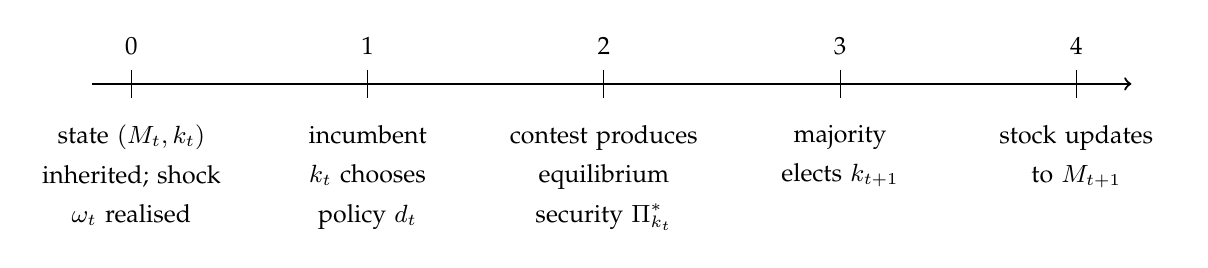
\begin{tikzpicture}[scale=1, font=\small]
\draw[->, thick] (-0.5, 0) -- (12.7, 0);
\foreach \x in {0,3,6,9,12}{
  \draw (\x, 0.18) -- (\x, -0.18);
}
\node[above] at (0, 0.25) {0};
\node[above] at (3, 0.25) {1};
\node[above] at (6, 0.25) {2};
\node[above] at (9, 0.25) {3};
\node[above] at (12, 0.25) {4};
\node[below, align=center, text width=2.4cm] at (0, -0.4) {state $(M_t,k_t)$ inherited; shock $\omega_t$ realised};
\node[below, align=center, text width=2.4cm] at (3, -0.4) {incumbent $k_t$ chooses policy $d_t$};
\node[below, align=center, text width=2.4cm] at (6, -0.4) {contest produces equilibrium security $\Pi^*_{k_t}$};
\node[below, align=center, text width=2.4cm] at (9, -0.4) {majority elects $k_{t+1}$};
\node[below, align=center, text width=2.4cm] at (12, -0.4) {stock updates to $M_{t+1}$};
\end{tikzpicture}
\caption{Timing.}
\label{fig:timing}
\end{figure}

The economy is a measure-one continuum of citizens divided into two ethnic or religious groups: a majority $\mathsf M$ of population share $n_M>1/2$, represented in the electoral arena by two competing parties $A$ (Hawk) and $B$ (Dove); and a minority $\mathsf m$ of share $n_m=1-n_M$, who do not vote.\footnote{In \suppmat, I relax this assumption to a strategic voting minority of arbitrary size $n_m\in(0,1/2)$ and characterises a three-regime partition of the Hawk's strategic problem. Specifically, I study 3 situations where minority is not pivotal. First, a small-$n_m$ regime in which the inverted-U electoral return shifts perturbatively. Then, an intermediate regime in which the inverted-U curve flattens. Thirdly, a corner regime ($n_m\ge\bar n_m$) in which the Hawk plays peace.} In each period the incumbent $k\in\{A,B\}$ commits to a policy vector $(d_k,g_k)\in\mathbb R_+^2$, where $d_k$ is the intensity of symbolic policy (cattle-slaughter bans, dress codes, citizenship registers, education policy, etc.) and $g_k$ is the level of public-good provision that shapes realised consumption.\footnote{I discuss the commitment problem of parties in \suppmat.} 
%The minority chooses mobilisation effort of resistance as the majority chooses enforcement effort, the contest plays out and voting happens, and the stock of minority mobilisation updates. 
The economy inherits state $(M_t,k_t)$ from the last period, the incumbent chooses policies, and contest starts off and each side yield effort. After the contest, the economy elects its party for the next period $K_{t+1}$, and $M_t$ updates to $M_{t+1}$, which is the post-contest minority mobilisation stock.
I first focus on a stylised two-period horizon with $M_1=0$ and $k_1=A$, and turn to the long-run dynamics by iterating the same primitives under i.i.d.\ salience shocks $\omega_t$ drawn from a continuous distribution $F$ with full support.

\paragraph{Voters.} 
Following retrospective-voting models \citep*{lindbeckBalancedbudgetRedistributionOutcome1987}, voter $i$'s per-period utility from incumbent $k\in\{A,B\}$ playing policy $d_k\ge 0$ at inherited stock $M$ is
\begin{equation}\label{eq:utility_v3}
    U^k(d_k;M)\;=\;\lambda\,\Pi_k^*(d_k,S_k;M)\;+\;(1-\lambda)\,u(\bar g_k)\;-\;\chi(d_k)\;+\;\mathbbm{1}[k=A]\,\nu_i,
\end{equation}
with $\lambda\in(0,1)$ the weight on security and $u(\cdot)$ strictly increasing. 
The first term is the equilibrium security delivered by the contest of \autoref{sec:block1} below. 
The second term is the (raw) economic-consumption utility, which the voter weights by $1-\lambda$. 
The third term captures the direct destruction that symbolic policy imposes on the economy, including policy implementation cost, lost productivity from communal segmentation, trade disruption, among other costs.
The destruction cost is continuously differentiable, strictly increasing, strictly convex, and satisfies $\chi(0)=0$ and $\lim_{d\uparrow\infty}\chi(d)=\infty$.
An idiosyncratic Hawk-bias $\nu_i$ drawn from a CDF $\Phi(\cdot)$ with median zero and a continuous, strictly positive density on $\mathbb R$. 

The voter's choice rule is \emph{myopic retrospective}. At each election, the voter observes the inherited stock $M_t$, and votes for whichever candidate would deliver higher per-period welfare under each party's best strategy at different realised state.\footnote{In \autoref{sec:block2}, I show $M_t$ summarises all prior contest history.} In the end of this section, I discuss alternative assumptions (e.g., forward-lookingness) of the voter. \suppmat~shows that the substantive results are robsut under MPE with discount factor $\delta\in(0,1)$.

%The voter's choice rule is \emph{myopic retrospective}: at every election she observes the inherited stock $M_t$, which summarises all prior contest activity, and votes for whichever candidate would deliver higher per-period welfare under each candidate's stationary best-reply at the realised state, adjusted for partisan bias. She does not solve a Bellman recursion. The Discussion below defends this assumption against the fully forward-looking alternative, and the \suppmat~shows that the substantive results survive under MPE with discount factor $\delta\in(0,1)$.

\paragraph{Parties.} The two competiting parties differ in a two-dimensional technological endowment $(S_k,\bar g_k)$:
\begin{equation}\label{eq:party_endowment_v3}
    S_A\;>\;S_B\quad\text{and}\quad\bar g_A\;<\;\bar g_B,
\end{equation}
so the Hawk has higher \emph{coercive capacity} and the Dove has higher \emph{economic capacity}. The pair $(S_k,\bar g_k)$ captures the coercive and the productive sides of state capacity, discussed in \citet*{besleyOriginsStateCapacity2009,besleyStateCapacityConflict2010}. However, I emphasis the comparative advantage of each party in one technology.
% two dimensions of state capacity discussed in \citet*{besleyOriginsStateCapacity2009,besleyStateCapacityConflict2010}, which are the coercive and the productive, on which the parties hold opposite comparative advantages. 
% I therefore refer to $S_k$ throughout as the party's \emph{coercive capacity}. 
These technological endowments are taken as primitives of party type. $S_k$, the coercive capacity, denotes bureaucratic expertise, legal framework, and party norms that sustain identity-related competition. 
$\bar g_k$ represents the organisational capacity in each party to deliver economic goods, which can be interpreted as coordinating ability for public goods (for example, infrastructure, education, etc.)  
These institutions are evolving slowly relative to a single electoral cycle, therefore can be treated exogenous.\footnote{In \autoref{sec:conclusion_v3}, I discuss how to relax these assumptions.}  
Voter utility is strictly increasing in $g$ and the ceiling $\bar g_k$ is the only constraint on the economic-policy margin, so every party finds it optimal to exhaust the technological frontier, $g_k^*=\bar g_k$, so $g$ carries no strategic effects in equilibrium. The (raw) economic deficit driving the Hawk's electoral handicap is therefore
\begin{equation}\label{eq:du_v3}
    \Delta u\;\equiv\;u(\bar g_B)-u(\bar g_A)\;>\;0,
\end{equation}
% the other face of the same comparative-advantage trade-off that gives the Hawk its higher coercive capacity.

I consider each party strategically choosing the symbolic-policy intensity $d_k\ge 0$ to maximise its retention probability over a one-cycle horizon. 
Each party takes into account of the voter's swing rule, and expects how its current policy translates into a next-election retention probability, through the updated stock $M_{t+1}$ which its current policy produces under contest. 
I discuss whether the one-cycle horizon is robust to fully strategic parties in the infinite-horizon setting below.

\paragraph{Contest.} Conflict in this economy is modelled as a two-sided Tullock contest between the majority and minority. The effort of each group is modelled as with-in group collective action game, in which citizens consider their effort strategically, given expectations on other citizens' effort.
%Each of them plays collective-action problems on both sides. 
Given aggregate efforts $(E_M,E_m)$ and the incumbent's competence $S_k$, the probability of majority dominance follows the Tullock contest success function (CSF)
\begin{equation}\label{eq:CSF_v3}
    \Pi_k(E_M,E_m)\;=\;\frac{S_k\,E_M}{S_k\,E_M+E_m}.
\end{equation}
Each member of the majority ($N_M$ in total) is identical. Each independently choose enforcement effort $e_i\ge 0$ at private cost $\tfrac{1}{2}e_i^2$ to maximise $\Lambda\Pi_k-\tfrac{1}{2}e_i^2$, where $\Lambda>0$ is the per-capita majority valuation of identity security. The interior FOC and the symmetric Nash condition ($e_i=e$) yield the following majority best-response
\begin{equation}\label{eq:EM_BR_v3}
    \frac{E_M}{N_M}\;=\;\Lambda\,\frac{S_k\,E_m}{(S_k E_M+E_m)^2}.
\end{equation}
Symmetrically, the minority consists of $N_m$ identical citizens, each choosing resistance effort $e_j\ge 0$ at private cost $\tfrac{1}{2\kappa}e_j^2$, where $\kappa>0$ denotes the minority's organisational capacity. The minority loses $\phi\,\hat d^\sigma$ from majority dominance, where $\phi>0$ is the grievance sensitivity and the total stake
\begin{equation}\label{eq:dhat_v3}
    \hat d^\sigma\;\equiv\;d^\sigma+\xi\,M,\qquad\sigma>0,\;\xi\ge 0,
\end{equation}
combines the current symbolic policy intensity and the inherited mobilisation stock through the policy-stake elasticity $\sigma$ and the stock-stake elasticity $\xi$. For $\xi$, high $\xi$ corresponds to long-memory polities in which inherited stock is heavy and any single period of provocation moves the perceived stake only slightly, with post-2014 India and post-1979 Iran as empirical examples.
Low $\xi$ features short-memory polities in which the stock channel is weak and current policy dominates, as in the post-2016 United States or post-Uribe Colombia. For the specific additive relationship I employed, I discuss its microfoundations in \autoref{subsec:discussion_v3}. Given these conditions, citizen $j$ therefore solves $\max_{e_j\ge 0}\,\phi\hat d^\sigma(1-\Pi_k)-\tfrac{1}{2\kappa}e_j^2$, which delivers the minority best-response
\begin{equation}\label{eq:Em_BR_v3}
    \frac{E_m}{N_m}\;=\;\kappa\phi\,\hat d^\sigma\,\frac{S_k\,E_M}{(S_k E_M+E_m)^2}.
\end{equation}
The two best-responses are structurally identical. The minority's optimal effort responds to the incumbent's technology $S_k$. Therefore, \autoref{lem:contest_v3} below characterises the joint equilibrium. Subsequently, the mobilisation stock then evolves at depreciation rate $\rho\in(0,1)$, with the following evolution law
\begin{equation}\label{eq:M_evolution_v3}
    M_{t+1}\;=\;(1-\rho)\,M_t\;+\;\rho\,E_m^*(d_t,S_{k_t};M_t),
\end{equation}
where $E_m^*(\cdot)$ is the within-period equilibrium minority effort and $M_0\ge 0$ is exogenous. 

\paragraph{Equilibrium properties.} The 2-period baseline contest is the symmetric Nash equilibrium of the joint within-group population game \citep*{sandholmPopulationGamesEvolutionary2010}, characterised by \autoref{lem:contest_v3} below.
The within-cycle equilibrium of the two-period game is solved with backward induction (\autoref{sec:block2}--\autoref{sec:block3}). 
The voter applies retrospective voting at the realised inherited stock $M_2$, and the Hawk's first-period policy maximises its period-2 retention probability internalizing voter's choice. 
The long-run equilibrium of the iterated game (\autoref{sec:dynamics_v3}) is the stationary perturbed-Markov-chain on $(M_t,k_t)$ generated by iterating the same swing rule and the same policy production problem of both parties subjected to the salience shock. The formal Markov-perfect formulation, with bounded $L^2$ strategy space and Glicksberg fixed-point existence, is discussed in \autoref{oa:mpe_v3}.

The within-cycle analysis (\autoref{sec:block1}--\autoref{sec:block3}) uses a stylised two-period game with $M_1=0$. The long-run analysis (\autoref{sec:dynamics_v3}) iterates the same primitives under the salience shock. One can read the two-period game as one cycle of the long-run iteration. \autoref{lem:hawk_t2_v3} then characterises the Hawk's stationary best-reply at any inherited stock, not necessarily at the period-2 settlement of a terminal cycle.

\subsection{ Discussion}\label{subsec:discussion_v3} 
I now discuss each substantive assumption, list the alternatives, and confess the trade-off.

\paragraph{Bounded rationality of voter and parties.} 

\emph{For the voter}, the empirical political-behaviour literature consistently argues that voters in low-information divided electorates use simple retrospective heuristics rather than infinite-horizon considerations. Therefore, the realised state $M_t$ is a sufficient statistic for prior contest activity \citep*{healyMyopicVotersNatural2009,achenDemocracyRealistsWhy2017}. 
\emph{For the Hawk}, the one-cycle horizon avoids commitment power that real-world hawkish parties do not possess, which is an incumbent who promises a long-horizon symbolic-policy path cannot bind successors.

\paragraph{The minority's mobilisation and electoral participation.} One may concern that a strategic minority leader could coordinate aggregate mobilisation downward in order to deny the Hawk. The \suppmat~addresses this concern as a Stackelberg-leader extension and shows that the only incentive compatibility (IC) consistent aggregate effort is the unconstrained Nash equilibrium of \autoref{lem:contest_v3}. The second concern is that the non-voting assumption intentionally silences the minority on the electoral margin. It is generally true that in most of examples we have covered earlier (\emph{India}, \emph{United States}, \emph{Taiwan}, and \emph{Iran}), the targeted minorities are never pivotal to elections. Nevertheless, the \suppmat~relaxes this assumption to a strategic voting minority of arbitrary share within $(0,1/2)$. 
I find the within-period contest equilibrium is $n_m$-invariant. 
%The Hawk's strategic-provocation problem partitions into three regimes in $n_m$: a small-$n_m$ perturbative regime, an intermediate distortion regime in which the inverted-U flattens, and a corner regime ($n_m$ above an explicit primitive threshold $\bar n_m$) in which the Hawk plays peace. 
In the long run, a joint function of $(\rho,n_m)$ separates the regime (persistence or cycle).\footnote{This corresponds to the empirical pattern in India, where the BJP cattle-ban intensity is lower in high-Muslim-share states (Assam, West Bengal, Kerala) than in low-Muslim-share states (the Hindi Belt, Gujarat, Maharashtra). In \suppmat,~I also show how does an active voting minority shapes the inverted-U curve between BJP vote share and social conflict.}
%With the trap region strictly decreasing in $n_m$ and collapsing to a peace equilibrium for $n_m\ge\bar n_m$ (see \autoref{sec:dynamics_v3}). 
I also verify that in \suppmat~that all qualitative content survives under fully forward-looking Markov-perfect equilibrium with discount factor $\delta\in(0,1)$.

% The cross-state empirical implication is that BJP cattle-ban intensity should be lower in high-Muslim-share states (Assam, West Bengal, Kerala) than in low-Muslim-share states (the Hindi Belt, Gujarat, Maharashtra), and the inverted-U-shaped vote-conflict mapping should be flatter in high-Muslim-share states, which is documented in \citet*{jaffrelotModisIndiaHindu2021}. Furthermore, Indian Muslims mobilised for the 2019--20 CAA protests and Iranian women mobilised after the 2022 Mahsa~Amini episode, both arguably strengthening the hard-line incumbent. Both episodes are consistent with the IC argument of the \suppmat and the perturbative regime of the \suppmat.

\paragraph{Additive contest stake.} 
I assume the augmented minority stake to be $\hat d^\sigma=d^\sigma+\xi M$. 
In \suppmat,~I provide three separate microfoundations for the additive form and conduct a robustness check with a more general CES form. 
For example, consider the minority updating their state as Bayedian agents. If the minority's prior on regime intent is $\theta_t\mid M_t\sim\mathcal{N}(M_t,\tau_M^{-1})$ with $\tau_M>0$ and the public signal is $s_t=d_t^\sigma+\epsilon_t$ with $\epsilon_t\sim\mathcal{N}(0,\tau_d^{-1})$, then $E[\theta_t\mid s_t,M_t]=(1-w)M_t+w\,d_t^\sigma$ with signal weight $w=\tau_d/(\tau_M+\tau_d)$ (distinct from the salience shock $\omega$ of \autoref{sec:dynamics_v3}), and rescaling by $1/w$ delivers $\hat d^\sigma=d^\sigma+\xi M$ with $\xi=\tau_M/\tau_d$.
%The augmented stake $\hat d^\sigma=d^\sigma+\xi M$ is the natural decomposition of two independent grievance sources, inherited organisational capital and fresh policy shock, each of which contributes independently to the minority's incentive to mobilise. 
%A multiplicative alternative ($d^\sigma\cdot\xi M$) would mechanically rule out residual mobilisation when current policy is zero, contradicting the lagged-dissipation pattern of \autoref{fig:rent_dissipation_event_study}. 
%A maximum alternative ($\max(d^\sigma,\xi M)$) loses smoothness and cannot generate the peak-shift result of \autoref{lem:invU_v3}. 
I also argue the additive form has two alternative independent microfoundations (organisational and adaptive learning), detailed in the \suppmat.~I also provides a CES-form robustness check, showing the qualitative results are consistent under any aggregator exponent $\psi\in[1,\infty]$. 

%with the peak-shift threshold $M^*=\alpha^2 S_AS_B/\xi$ itself $\psi$-invariant.

% \paragraph{The stock-stake elasticity at the polity level.} 

% The same information-flow regime that lets historical episodes anchor today's perceived stake also lets organisational and identity-salience capital persist across periods, so $\xi$ tends to co-vary inversely with $\rho$ across polities. This co-variation tightens the long-run mapping in \autoref{sec:dynamics_v3} but is not a primitive of the formal analysis.

%\paragraph{Two-period exposition versus iterated long run.} 

%The within-cycle analysis (\autoref{sec:block1}--\autoref{sec:block3}) uses a stylised two-period game with $M_1=0$ for clean backward induction. The long-run analysis (\autoref{sec:dynamics_v3}) iterates the same primitives under the salience shock. The reader who prefers can read the two-period game as one cycle of the long-run iteration; \autoref{lem:hawk_t2_v3} then characterises the Hawk's stationary best-reply at any inherited stock, not specifically at the period-2 settlement of a terminal cycle.

\paragraph{Tullock contest specification.} 
Following theoretical literature in contest theory, I adopt the Tullock CSF for baseline analysis. The literature assumes performance levels $Y_M=\ln(S_kE_M)+\varepsilon_M$ and $Y_m=\ln(E_m)+\varepsilon_m$ with i.i.d.\ Gumbel errors. The probability of majority dominance simplifies to \eqref{eq:CSF_v3} \citep*{skaperdasContestSuccessFunctions1996,jiaStochasticDerivationRatio2008}. However, my model micro-found the effort with collective-action problems within each group, contrasting prior contest models typically treat groups as unitary actors. The model also features asymmetric stake structure. Specifically, my model features contest over identity security, with different majority parties holding different coercive capacity $S_k$. On the other sides, the minority's effort follows augmented contest stake $\hat d^\sigma$. These within-group features in the model makes the symbolic policy a strategic instrument for the subsequent electoral game.


% The Tullock CSF  is the workhorse of contest theory and admits a closed-form Nash equilibrium under within-group collective action. It can be derived as the probability of majority dominance under a generalised Logit microfoundation \citep*{jiaStochasticDerivationRatio2008}. The two-sided structure with within-group collective-action problems on both sides is the model's key formal innovation, since prior contest models typically treat groups as unitary actors. The asymmetric stake structure, in which the majority cares about dominance while the minority cares about resistance and its stake scales in the augmented contest stake $\hat d^\sigma$, is what makes the Hawk's symbolic policy a strategic instrument in the electoral game.

\section{The Contest}\label{sec:block1}

Following \autoref{sec:model_v3}, I characterise the witnin-period equilibrium of the contest. Specifically, I define the joint mobilisation problem of the majority and the minority. Then, I define the security provided by each party under such mobilisation efforts, and show its comparative statistics with regards to party's coercive capacity. I study the properties of security premium $\Delta\Pi(d;M)$ that Hawk obtains over Dove. I continue to define the rent dissipation in the contest, which can be interpreted as the aggregated conflict.

%This section characterises the within-period equilibrium of the contest set up in the Contest paragraph of \autoref{sec:model_v3}: the joint mobilisation of the majority and the minority, the closed-form security delivered by each party, the comparative statics in coercive capacity, the security premium with its shifting peak, and the resulting rent dissipation. The output is a closed-form security premium $\Delta\Pi(d;M)$ that the electoral analysis of \autoref{sec:block2}--\autoref{sec:block3} takes as a primitive.

\subsection{Joint contest equilibrium}\label{subsec:contest_eqm_v3}

The joint contest equilibrium conditional on $(d,S_k,M)$ is the pair $(E_M^*,E_m^*)$ pinned down by (\ref{eq:EM_BR_v3}, majority best response) and (\ref{eq:Em_BR_v3}, minoirty best response) defined above. 
In the next lemma, I characterise this equilibrium and how does it change with incumbent's coercive capacity and the intensity of symbolic policy. 
For every current symbolic policy and inherited stock, the within-period subgame admits a unique symmetric Nash equilibrium.
The inherited mobilisation stock enters this equilibrium only through the augmented stake $\hat d^\sigma$. 
Effort on both side is 0 (contest is dormant) if and only if both current symbolic policy and the inherited stock are both zero.
Equilibrium security is strictly increasing in the incumbent's coercive capacity and strictly decreasing in the augmented stake.

%Define the technology-independent stakes ratio $\alpha\equiv\sqrt{\Lambda N_M/(\kappa\phi N_m)}$ and the scale constant $\beta\equiv(\kappa\phi N_m\Lambda N_M)^{1/4}$. The joint contest equilibrium conditional on $(d,S_k,M)$ is the pair $(E_M^*,E_m^*)$ that simultaneously satisfies \eqref{eq:EM_BR_v3} and \eqref{eq:Em_BR_v3}. The next lemma characterises this equilibrium in closed form and isolates the two comparative statics that the electoral analysis will use.

\begin{lemma}[\emph{Joint contest equilibrium}]\label{lem:contest_v3}
Fix $(d,S_k,M)\in[0,\infty)\times(0,\infty)\times[0,\infty)$ and define $\hat d^\sigma\equiv d^\sigma+\xi M$. Define the stake ratio $\alpha\equiv\sqrt{\Lambda N_M/(\kappa\phi N_m)}$ and the scale constant $\beta\equiv(\kappa\phi N_m\Lambda N_M)^{1/4}$ (note these contests are independent to contest technology). 
The contest is dormant ($E_M^*=E_m^*=0$ and $\lim_{\hat d\downarrow 0}\Pi_k^*=1$) if $\hat d^\sigma=0$.
On the other hand, if $\hat d^\sigma>0$, the unique equilibrium admits
\begin{equation}\label{eq:Em_Sk_explicit_v3}
    E_m^*(d,S_k;M)\;=\;\frac{\beta\,S_k^{1/2}\,\hat d^{\,3\sigma/4}}{S_k\alpha+\hat d^{\,\sigma/2}},
    \qquad
    E_M^*(d,S_k;M)\;=\;\alpha\,\beta\,\frac{S_k^{1/2}\,\hat d^{\,\sigma/4}}{S_k\alpha+\hat d^{\,\sigma/2}},
\end{equation}
with equilibrium effort ratio $E_M^*/E_m^*=\alpha\,\hat d^{-\sigma/2}$ and security
\begin{equation}\label{eq:Pi_v3}
    \Pi_k^*(d,S_k;M)\;=\;\frac{S_k\alpha}{S_k\alpha+\hat d^{\,\sigma/2}},
\end{equation}
both strictly increasing in $S_k$, strictly decreasing in $\hat d$, $\lim_{\hat d\downarrow 0}\Pi_k^*=1$, and $\lim_{\hat d\uparrow\infty}\Pi_k^*=0$.
\end{lemma}

The proof is in \autoref{app:proofs_v3}.
\autoref{lem:contest_v3} offers the following intuition of contest in equilibrium. The majority-minority effort ratio is not related to coercive technology, because the incumbent's coercive capacity shifts the level of effort from both sides simultaneously but not their ratio. Also, security provision is monotone in both coercive technology and symbolic policies. Here, Hawk's higher coercive capacity benefits both directly and indirectly. With the same effort, higher coercive capacity from Hawk magnifies the majority effort $S_A$ (larger than $S_B$) times (direct channel). Moreover, because the direct channel raises the private return of majority mobilisation, equilibrium majority effort under Hawk is as well higher then Dove (indirect channel). Lastly, peaceful condition requires both symbolic policy and inherited mobilisation to be 0. Therefore, a Dove who inherits a high stock from a previous Hawk cannot ``unwind" the contest quickly. 

%\autoref{lem:contest_v3} leads to three key interpretations. First, the majority-to-minority effort ratio $\alpha\hat d^{-\sigma/2}$ does not depend on $S_k$: the incumbent's coercive capacity shifts the level of both efforts but not their ratio. Second, security is monotone in both arguments and the Hawk's higher $S_A$ dominates the level of effective enforcement throughout. Third, dormancy requires both $d=0$ and $M=0$. The inherited stock alone keeps the contest active even after a Hawk-to-Dove transition, so a Dove who inherits a high stock from a previous Hawk regime cannot ``unwind'' the contest by enacting counter-symbolic policy. It can only set $d=0$ and wait for $M$ to decay at rate $\rho$. The proof is in \autoref{app:proofs_v3}.

\subsection{State capacity, mobilisation, and effective enforcement}\label{subsec:Sk_v3}

\autoref{lem:contest_v3} asks when the contest intensifies (i.e., grievance stock increases or policies become more radical), and the same party is in power, how do the effort levels and security in the equilibrium change. Now, I turn to the following question: how do equilibrium objects above change conditional on contest strength remaining constant while different parties are elected (i.e., from Dove's low $S_B$ to Hawk's high $S_A$). The following lemmas shows when holding the augmented stake fixed, raw mobilisation is single-peaked in coercive capacity. Effective enforcement and equilibrium security rise monotonically with regards to coercive capacity. A more coercive incumbent first encourages street-level enforcement, but then progressively substitutes its own coercive apparatus for it.

%encodes the joint dependence of the equilibrium on the contest stake and on coercive capacity. The discussion above traced its behaviour across stakes at any given coercive capacity. The dual comparative-static slice runs in the other direction: how do mobilisation, effective enforcement, and equilibrium security each vary with coercive capacity at fixed stake?

\begin{lemma}[\emph{Coercive capacity and mobilisation}]\label{lem:Sk_v3}

Fix $\hat d>0$. Both $E_M^*$ and $E_m^*$ are continuously differentiable and strictly positive on $S_k\in(0,\infty)$, and both are single-peaked in $S_k$ with common unique maximiser
\begin{equation}\label{eq:Sk_threshold_v3}
    \overline S(\hat d)\;\equiv\;\hat d^{\sigma/2}/\alpha.
\end{equation}
Effective majority enforcement $Z_k^*\equiv S_k E_M^*$ and equilibrium security $\Pi_k^*$ are strictly increasing in $S_k$ on $(0,\infty)$. At $S_k=\overline S(\hat d)$ the contest is exactly symmetric ($\Pi_k^*=1/2$) and peak majority mobilisation is
\begin{equation}\label{eq:EM_peak_v3}
    E_M^*\big(\hat d,\overline S(\hat d)\big)\;=\;\tfrac12\sqrt{\Lambda N_M},
\end{equation}
independent of $\hat d$ and primitives.
\end{lemma}

The proof is in \autoref{app:proofs_v3}.
\autoref{lem:Sk_v3} demonstrates the strategic substitutability/complementarity between top-down coercive capacity of the party (eg., police force, etc.) and the bottom-up decentralised enforcement from the citizens (e.g., identity-related protest or violence). When party's coercive capacity is low, decentralised enforcement has little leverage in the contest, and free-riding dominates and mobilisation is weak. When coercive capacity rises, each unit of citizen effort becomes more effective and the private return to participation increases. In the intermediate range of $S_k$, for the incumbent party to maintain its contest advantage, it must rely on grassroot mobilization, rather than solely on its own coercive power. In this range, an increase in $S_k$ leads to an increase in mass mobilization $E_M$, with the two mutually reinforcing each other rather than substituting for one another. Once $S_k$ exceeds $\overline S(\hat d)$, the incumbent's coercive apparatus is sufficiently effective that dominance can be maintained with less decentralised effort, the private return falls, and citizens subsequently withdraw. 

In \autoref{fig:Sk_statics}, Panel~(A) shows the inverted-U relationship between coercive capacity (top-down) and majority's mobilisation (bottom-up). Panel~(B) demonstrates the monotonic relationship between coercive capacity and effective mobilisation (top-down coercive capacity times bottom-up mobilisation). This matches \autoref{fact:3} introduced in \autoref{sec:empirical_facts}. In India, the most intense ground-level enforcement appears in states with intermediate, not maximal, BJP institutional capacity (see \citet*{jaffrelotModisIndiaHindu2021}, \citet*{mitraImplicationsEconomicTheory2014}, and map shown in \autoref{fig:maps}).


%When $S_k$ is low, decentralised enforcement has little leverage in the contest, so free-riding dominates and mobilisation is weak. As $S_k$ rises into an intermediate range, each unit of citizen effort becomes more effective and the private return to participation rises; in this region a Hawk that is stronger than the Dove but not overwhelmingly strong relies on grass-roots enforcement, and coercive capacity \emph{complements} citizen mobilisation. Once $S_k$ exceeds $\overline S(\hat d)$, the incumbent's coercive apparatus is sufficiently effective that dominance can be maintained with less decentralised effort, the private return falls, and citizens withdraw. \autoref{fig:Sk_statics} plots both panels, and the spatial heterogeneity of cattle-ban mobilisation in \autoref{fig:maps} matches the theoretical prediction: the most intense ground-level enforcement appears in states with intermediate, not maximal, BJP institutional capacity. The proof is in \autoref{app:proofs_v3}.

% --- Figure fig:Sk_statics inlined here ----------------------------------
% Moved out of the trailing Figures section per supervisor request.
\begin{figure}[!h]
    \centering
    \subfigure[\bf majority mobilization peaks at $S_k=\overline{S}(E_m)$.]{%
        
\includegraphics[width=0.48\textwidth]{fig_Sk_statics_mobilization.jpg}%
        \label{fig:Sk_statics_mobilization}%
    }\hfill
    \subfigure[\bf Effective enforcement $Z_k^*$ keeps rising beyond the mobilization peak.]{%
        
\includegraphics[width=0.48\textwidth]{fig_Sk_statics_enforcement.jpg}%
        \label{fig:Sk_statics_enforcement}%
    }
    \caption{\normalsize\bf Coercive capacity, street mobilization, and effective enforcement.}
    \label{fig:Sk_statics}
    \floatfoot*{\footnotesize\textit{Notes}: The left subfigure plots the symmetric equilibrium $E_M^*(d,S_k)$ from \eqref{eq:Em_Sk_explicit_v3} against relative coercive capacity $S_k/\overline{S}(d)$, where $\overline{S}(d)=d^{\sigma/2}/\alpha$ is the threshold from \autoref{lem:Sk_v3}. To the left of the threshold, higher coercive capacity raises the return to decentralized participation and increases majority mobilization; to the right, stronger coercive capacity substitutes for street-level effort and $E_M^*$ declines. The right subfigure plots effective enforcement $Z_k^*=S_kE_M^*(d,S_k)$ over the same range. Because $Z_k^*$ keeps rising after the peak in $E_M^*$, higher-capacity regimes can generate more effective control with less visible mass participation. The marked points illustrate a low-capacity Dove, an intermediate-capacity Hawk below the threshold, and a stronger Hawk above the threshold. Parameters are $(N_M,N_m,\Lambda,\kappa,\phi,\sigma,d)=(100,100,1,1,1,1,1)$.}
\end{figure}
% ----------------------------------------------------------------------

\subsection{The single-peaked security premium}\label{subsec:invU_v3}

Now I turn to how the security provision in equilibrium varies with current symbolic policy. Following \citet{barutSymmetricMultiplePrize1998}, I define the security premium
%The substantively important comparative static for the electoral analysis is how the closed-form security $\Pi_k^*$ varies with current symbolic policy when the two parties are evaluated at a common environment $(d,M)$. Following \citet{barutSymmetricMultiplePrize1998}, I define the security premium
\begin{equation}\label{eq:security_premium_v3}
    \Delta\Pi(d;M)\;\equiv\;\Pi_A^*(d,S_A;M)-\Pi_B^*(d,S_B;M)
    \;=\;\frac{S_A\alpha}{S_A\alpha+\hat d^{\,\sigma/2}}-\frac{S_B\alpha}{S_B\alpha+\hat d^{\,\sigma/2}}.
\end{equation}
which is single-peaked in current symbolic policy and attains a ceiling that depends only on the technology ratio. As the inherited stock $M$ rises, the position of this peak shifts leftward along the $d$-axis. Once $M$ crosses the threshold $\alpha^2 S_A S_B/\xi$, the optimal current symbolic policy is $d=0$ (i.e., paradox of restraint). Any additional $d$ at that point would push the security premium into its decreasing branch. \autoref{lem:invU_v3} formalises the intuition.

\begin{lemma}[\emph{Security premium}]\label{lem:invU_v3}
\emph{}
Suppose $S_A>S_B>0$. Then $\Delta\Pi(\,\cdot\,;M)$ is single-peaked on $[0,\infty)$ for each $M\ge 0$, with maximiser
\begin{equation}\label{eq:dpeak_v3}
    d^{\mathrm{peak}}(M)\;=\;\begin{cases}
        \big(\alpha^2 S_A S_B-\xi M\big)^{1/\sigma} & \text{if }M<\alpha^2 S_A S_B/\xi,\\[2pt]
        0 & \text{if }M\ge\alpha^2 S_A S_B/\xi.
    \end{cases}
\end{equation}
For $M<\alpha^2 S_A S_B/\xi$ the unconstrained peak attains the technology-ratio ceiling
\begin{equation}\label{eq:DPi_peak_v3}
    \max_{d\ge 0}\Delta\Pi(d;M)\;=\;\frac{\sqrt{S_A}-\sqrt{S_B}}{\sqrt{S_A}+\sqrt{S_B}}\;\in\;(0,1),
\end{equation}
For $M\ge\alpha^2 S_A S_B/\xi$, $\Delta\Pi(\cdot;M)$ is strictly decreasing in $d$ on $[0,\infty)$, and the constrained maximum is attained at $d=0$ with value $\Delta\Pi(0;M)<(\sqrt{S_A}-\sqrt{S_B})/(\sqrt{S_A}+\sqrt{S_B})$, with $\Delta\Pi(0;M)>0$ for all $M>0$.
\end{lemma}

The proof is in \autoref{app:proofs_v3}.
\autoref{lem:invU_v3} delivers the following intuition. At $M=0$ the optimal symbolic policy sits at $d^{\mathrm{peak}}(0)=(\alpha^2 S_A S_B)^{1/\sigma}$ and \eqref{eq:DPi_peak_v3} reproduces the static-benchmark ceiling seen in \autoref{sec:block1}. 
%For any technology pair, the Hawk's contest-based electoral advantage is bounded above by $(\sqrt{S_A}-\sqrt{S_B})/(\sqrt{S_A}+\sqrt{S_B})$, depending only on the ratio $S_A/S_B$ and structurally independent of how grievance-elastic the minority is, how large the two populations are, or how the majority's collective-action problem scales. 
For any technology pair, the Hawk's contest-based electoral advantage is bounded by $(\sqrt{S_A}-\sqrt{S_B})/(\sqrt{S_A}+\sqrt{S_B})$.
One can find this ceiling depends only on the ratio $S_A/S_B$ and is invariant to other structural variables including minority's response elasticity in symbolic policies and population levels. 
Empirically, this means one can predict the ceiling of symbolic provocation based on the coercive technology ratio between the two parties in each country.
Moreover, as the inherited stock $M$ grows toward the threshold $\alpha^2 S_A S_B/\xi$, the peak moves leftward along the $d$-axis. 
Every unit of inherited mobilisation substitutes current provocation, so the Hawk needs less new symbolic provocation to reach the same contest activation. 
Consequently, any current $d>0$ moves the system into the decreasing branch of the inverted-U shape. 
In this case, the Hawk's optimum is then the corner $d=0$. 
Later, I will how does the intuition here affects the Hawk's optimal period-2 reaction in \autoref{lem:hawk_t2_v3}(paradox of restraint).

The proof is in \autoref{app:proofs_v3}.
The second intuition is that the within-period security gap is strictly positive even at $d=0$ whenever $M>0$.
Even if the Dove takes office and chooses $d_B=0$, the Hawk's $S_A$-advantage remains electorally salient through the inherited stock.
This rationalises the post-2014 BJP's continued electoral resilience even in periods (e.g.\ around demonetisation) when no new cattle-ban legislation was being enacted. 
\autoref{fig:reaction_functions} plots $\Delta\Pi(d;M)$ for different values of $M$, showing the shifting peak of minority mobilisation. 
Empirically, this corresponds to \autoref{fig:security_premium_empirical} that shows the relationship between ban intensity with BJP vote share (see \autoref{fact:3} in \autoref{sec:empirical_facts}). 
%The leftward shift of the peak past the point at which further provocation reduces the Hawk's advantage shows that non-targeted top-down interventions can entrench, rather than dampen, the very contested norm they target. 
Hawk's security premium peak shifts to the left as its inherited stock $M$ rises. At a certain point, new policies $d$ can weaken Hawk's own advantage. 
This shows when governments top-down policy measures to regulate symbolic policies (eg., banning cattle-slaughter bans), such policies may end up solidify the conflict rather than suppress it. In \autoref{sec:conclusion_v3}, I discuss why top-down policies may backfire due to the manufacturing enemies with social identity.


% --- Figure fig:reaction_functions inlined here ----------------------------------
% Moved out of the trailing Figures section per supervisor request.
\begin{figure}[!h]
    \centering
    
\includegraphics[width=0.92\textwidth]{fig_reaction_functions.jpg}
    \caption{\normalsize\bf Security Premium and the Provocation Ceiling.}
    \label{fig:reaction_functions}
    \floatfoot*{\footnotesize\textit{Notes}: The figure plots the security premium $\Delta\Pi(d)=\Pi_A^*(d,S_A)-\Pi_B^*(d,S_B)$ from \eqref{eq:security_premium_v3} as a function of symbolic policy intensity $d$, for a Hawk-Dove pair with $S_A>S_B$. The curve is zero at $d=0$ (dormant contest: both parties deliver full dominance), rises on $(0,d^{\mathrm{peak}})$ as symbolic policy activates the contest and exposes the Hawk's technological advantage, and falls on $(d^{\mathrm{peak}},\infty)$ as further provocation erodes realized security for both parties. The peak value $(\sqrt{S_A}-\sqrt{S_B})/(\sqrt{S_A}+\sqrt{S_B})$ depends only on the technology ratio $S_A/S_B$. Illustration uses $(N_M,N_m,\Lambda,\kappa,\phi,\sigma,S_A,S_B)=(100,100,1,1,1,1,1.0,0.4)$.}
\end{figure}
% ----------------------------------------------------------------------

\subsection{Rent dissipation}\label{subsec:RD_v3}

The contest is costly. To track the cost of the contest, I define resource waste by the sum of equilibrium efforts (rent dissipation) in preserving identity security, define
\begin{equation}\label{eq:RD_v3}
    RD(d,S_k;M)\;\equiv\;E_M^*(d,S_k;M)+E_m^*(d,S_k;M)\;=\;\big(1+\alpha\,\hat d^{-\sigma/2}\big)\,E_m^*(d,S_k;M).
\end{equation}
where \autoref{fig:rent_dissipation} plots $RD(d,S_k)$ across symbolic policy intensities for two different levels of coercive capacity, and motivates the following proposition.
% , illustrating how the activated contest expends real resources on both sides.


% --- Figure fig:rent_dissipation inlined here ----------------------------------
% Moved out of the trailing Figures section per supervisor request.
\begin{figure}[!h]
    \centering
    
\includegraphics[width=0.88\textwidth]{fig_rent_dissipation.jpg}
    \caption{\normalsize\bf Rent dissipation under symbolic policy.}
    \label{fig:rent_dissipation}
    \floatfoot*{\footnotesize\textit{Notes}: The figure plots $RD(d,S_k)$ from \eqref{eq:RD_v3} as a function of symbolic policy intensity $d$, for two levels of coercive capacity. Symbolic policy activates the joint contest in \autoref{lem:contest_v3}, generating real resource dissipation through both minority mobilization and majority enforcement. Unlike the neutral contest designer in standard contest models (e.g., \citet{barutSymmetricMultiplePrize1998}), the political incumbent may optimally choose a strictly positive $d$, and hence positive dissipation, because conflict increases the security premium in elections. Parameters are $(N_M,N_m,\Lambda,\kappa,\phi,\sigma,S_A,S_B)=(100,100,1,1,1,1,1.0,0.2)$.}
\end{figure}
% ----------------------------------------------------------------------

\begin{proposition}[\emph{Persistence of rent dissipation}]\label{prop:RD_v3}
Equilibrium rent dissipation is strictly positive whenever the minority's augmented mobilisation stake is positive, so contest waste persists even after a Hawk-to-Dove transition through the stock channel alone.
Formally, for any $S_k>0$, $RD(d,S_k;M)>0$ whenever $\hat d^\sigma>0$ (i.e., whenever either $d>0$ or $M>0$). Particularly, even Dove-incumbent regimes ($d_B=0$) at $M>0$ generate strictly positive contest dissipation.
\end{proposition}

The proof is in \autoref{app:proofs_v3}. In the static benchmark, switching from Hawk to Dove instantly eliminates the contest's resource cost because $d_B=0$ collapses both efforts to zero. However, this is no longer the case if mobilisation follows the stock. A Dove inheriting $M>0$ continues to bear positive enforcement and resistance effort costs until the stock decays. In \autoref{fact:4} of \autoref{sec:empirical_facts}, \autoref{fig:rent_dissipation_event_study} shows this lagged dissipation pattern in the voilence data of India. Post-adoption ban effects on Hindu--Muslim violent events are positive and persistent for at least ten years across all four bovine-family ban types. The proposition therefore provides the model-level explanation for the empirical persistence of communal violence, even after change in political power. This also matches the long-run persistence in voilence even after regime change \citep*{acemogluSocialStructureDevelopment2011,voigtländerPersecutionPerpetuatedMedieval2012,luRobotInsurgencySocialist2024}. The mechanism therefore decouples observed communal violence from the timing of fresh legislation. violent events stay elevated for years after a state's first ban, even in years and states in which no further ban legislation is enacted.

\section{The Election}\label{sec:block2}

I now turn to the period-2 election, conditional on the inherited minority mobilisation stock realised in the contest characterised in \autoref{sec:block1}. Once again, voters follow a myopic-retrospective decision based on \eqref{eq:utility_v3}, \autoref{sec:model_v3}. Specifically, the voter chooses from a Dove who is technologically-desadvantaged to defend against mobilised monority, and a Hawk is technologically-advanced in identity but may expose voters to economic disruption. 

%I now solve the period-2 election conditional on an inherited grievance stock $M_2$, taking the voter utility \eqref{eq:utility_v3} of the Voters paragraph in \autoref{sec:model_v3} as a primitive. This is the analytical heart of the paper. The voter compares two scenarios: a Dove who is structurally unable to contain the inherited grievance, and a Hawk who would contain it but at the cost of real economic destruction. The Hawk's stationary best-reply, the swing-voter equation that decides the election, and the paradox of restraint all emerge from a single trade-off.

\subsection{The Dove's dominant strategy}\label{subsec:dove_v3}

Dove's choice is trivial. If Dove wins the election, it will choose the intensity of symbolic policy strength $d_B \geq 0$ to maximize voters' current utility. However, if $d_B > 0$, (1) Dove's own security $\Pi_B^*$ will decrease (because adding policy will activate minority mobilization, and Dove does not have Hawk's coercive advantage $S_B < S_A$, so contest activation will only lower Dove's winning prospect in elections). (2) Destruction cost $\chi(d_B)$ will increase (symbolic policies themselves have economic and social costs). Both forces act against the Dove at any inherited stock. Therefore, the Dove's unique best response is to set period-2 symbolic policy to zero, regardless of inherited grievance. I conclude the intuition with the following lemma.

% Under the unified utility \eqref{eq:utility_v3}, the Dove's period-2 problem is particularly simple. Should it win, it chooses $d_B\ge 0$ to maximise the voter's per-period utility (which is what the voter will compare across scenarios when forming its period-2 vote). A positive $d_B$ simultaneously reduces the Dove's equilibrium security $\Pi_B^*(d_B,S_B;M_2)$ (\autoref{lem:contest_v3}) and raises the destruction cost $\chi(d_B)$. Both forces work against the Dove at any inherited stock.

\begin{lemma}[\emph{Dove's dominant strategy}]\label{lem:dove_v3}
% \emph{The Dove's unique best response is to set period-2 symbolic policy to zero, regardless of inherited grievance: it gains no contest advantage from activating the security dimension, and it would only add to the destruction the voter is being asked to weigh.}
Suppose the Dove is the period-2 incumbent at inherited stock $M_2\ge 0$. Then $d_B^*(M_2)=0$ for all $M_2\ge 0$. The joint contest under Dove incumbency at $t=2$ is dormant if and only if additionally $M_2=0$, and is otherwise sustained purely by the inherited stock.
\end{lemma}

The proof is in \autoref{app:proofs_v3}. In \autoref{lem:dove_v3}, the Dove's solution is an endogenous equilibrium outcome. Any positive $d_B$ the Dove plays would simultaneously widen the security premium in the Hawk's favour and bear a destruction cost the voter would punish. Moreover, this result holds for any $M_2\ge 0$. A Dove who inherits a high stock from a previous Hawk cannot deactivate the contest by enacting counter-symbolic policy. In contrast, the Dove can only set $d_B=0$ and wait for the stock to decay at rate $\rho$ via \eqref{eq:M_evolution_v3}. The lagged-dissipation pattern of conflict in \autoref{fact:4} (\autoref{fig:rent_dissipation_event_study}) is consistent with the intuition that even Dove takes the office, it is still not able to deactivate an already-mobilised contest in the short run. 

\subsection{The Hawk's stationary best-reply and the paradox of restraint}\label{subsec:hawk_t2_v3}

Conditional on having won the election, the Hawk's period-2 problem is to choose the intensity of symbolic-policy that maximises the security premium it will have within the next cycle net of the economic destruction its own current provocation imposes on voters.
%I read $t=2$ as the start of the next electoral cycle in a stationary iteration of the same primitives: the Hawk-incumbent's reaction at any inherited stock $M$ is the policy that maximises its electoral signal at that stock, recognising that voters will eventually weigh the same trade-off in the next election they face. Formally, it solves
$t=2$ is the starting point of the next election cycle, therefore, the model repeats the same primitive repeating round after round. Hawk's symbolic policy intensity, chosen under any inherited stock $M$, is the same stationary best-reply function. Here, Hawk only considers the current $M$, regardless of the specific election cycle. Hawk knows that voters will use the same voter trade-off in $t+1$, $t+2$, etc., so the optimal response is simply a function of $M$. Formally, Hawk solves for
\begin{equation}\label{eq:hawk_t2_objective_v3}
    d_A^*(M_2)\;\equiv\;\arg\max_{d_A\ge 0}\;\big\{\,\lambda\,\Delta\Pi(d_A;M_2)\;-\;\chi(d_A)\,\big\},
\end{equation}
the security premium of \eqref{eq:security_premium_v3} net of the destruction cost.
%The Hawk's optimal symbolic policy is non-increasing in the inherited stock and reaches the corner once the stock alone has pushed the contest past its inverted-U peak. A sufficiently entrenched Hawk regime therefore governs without enacting visibly new symbolic policy, not because it has moderated its preferences but because the stock it manufactured in the previous cycle is doing the contest-activation work for it.
A Hawk regime that has become deeply entrenched may find itself in a state of governing but not enacting new laws. This is because the grievance stock it generated in the previous cycle has already activated the contest for it.
Therefore, Hawk's optimal symbolic policy does not increase as inherited stock $M$ rises (it will only remain flat or decrease). 
Once $M$ has pushed the contest past the peak of inverted-U, Hawk's optimal policy drops directly to corner solution $d_A^ = 0$*.
The next lemma characterises Hawk's best reaction as a strategic party.

\begin{lemma}[\emph{Hawk's stationary best-reply}]\label{lem:hawk_t2_v3}
Under the regularity conditions on $\chi$ stated alongside \eqref{eq:utility_v3}, supplemented by either (i) $\sigma<1$ (so that $\partial\hat d^\sigma/\partial d\to\infty$ as $d\downarrow 0$, an Inada condition that guarantees an interior maximiser on the shallow branch for any finite $\chi'(0)$) or (ii) $\sigma=1$ together with $\chi'(0)<\lambda h'(\sqrt{\xi M_2})/(2\sqrt{\xi M_2})$ on the shallow branch, the unique maximiser $d_A^*(M_2)$ of \eqref{eq:hawk_t2_objective_v3} satisfies
\begin{equation}\label{eq:dA_t2_v3}
    d_A^*(M_2)\;\begin{cases}
    \;>\;0 \text{ and is strictly decreasing in }M_2 & \text{for }M_2<\alpha^2 S_A S_B/\xi,\\[2pt]
    \;=\;0 & \text{for }M_2\ge\alpha^2 S_A S_B/\xi.
    \end{cases}
\end{equation}
In the deep regime the entire economic destruction is avoided ($\chi(d_A^*(M_2))=0$), and the Hawk delivers $\Pi_A^*(0,S_A;M_2)$, strictly above the Dove's $\Pi_B^*(0,S_B;M_2)$ at the same $M_2$. The maximum value of the objective in \eqref{eq:hawk_t2_objective_v3} is continuous in $M_2$ and single-peaked at the peak-shift threshold.
\end{lemma}

%\autoref{lem:hawk_t2_v3} is consistent with the model's explanation for the post-2014 plateau in headline cattle-ban legislation alongside sustained electoral majorities visible in \autoref{fig:cycles_four_panel}. 
The proof is in \autoref{app:proofs_v3}.
\autoref{lem:hawk_t2_v3} explains a seemingly paradoxical phenomenon in India after 2014: the BJP has enacted fewer and fewer new cattle-slaughter bans, yet it hasn't lost any votes (\autoref{fact:2},
  \autoref{fig:cycles_four_panel}).
%Once the inherited grievance stock has exceeded the threshold $\alpha^2 S_A S_B/\xi$, marginal provocation moves $\Delta\Pi$ into its decreasing branch (\autoref{lem:invU_v3}) while still adding to economic destruction. 
once the accumulated grievance stock $M$ exceeds a certain threshold, any further new policies by the BJP would result in losses on both ends. Consequently, the security premium would start to decline (having passed the single pick), but the destruction cost would continue to rise. Both forces prevent the Hawk from taking further action.
Both forces push the Hawk to the corner solution $d_A^*=0$. However, this does not mean the Hawk has lost its advantage in technology. The remaining $M$ continues to allow the minority to mobilize, so the security gap between Hawk and Dove remains positive. 

Empirically, this represents the post-2014 BJP arc visible in \autoref{fig:cycles_four_panel}. Peak rhetorical and legislative activity around 2014--19 corresponds to the period-1 provocation, while the visible plateau in headline cattle-ban legislation in 2020--24 corresponds to the period-2 settlement at the corner, even as cumulative ban intensity (\autoref{fig:policy_cumulative_rollout}) and communal-violence intensity (\autoref{fig:maps} panel B) remain at their elevated levels because the inherited stock has not decayed.
%It still delivers a strictly positive security premium $\Pi_A^*(0,S_A;M_2)-\Pi_B^*(0,S_B;M_2)>0$ purely through the persistence of $M_2$ on the minority side, but it does so without paying any fresh destruction cost. 
Therefore, we observe that even if legislation policies is decreasing, but communal mobilization underneath conflict has been continued (\autoref{fact:4}, \autoref{fig:rent_dissipation_event_study}). 
% \textcolor{red}{The same channel operates after Hawk-to-Dove transitions: by \autoref{lem:dove_v3} the Dove sets $d_B=0$, while by \autoref{prop:RD_v3} the contest continues to dissipate at rate $\rho$ purely through the inherited stock, so observed communal mobilisation does not track the visible quantity of fresh policy.}
%The empirical signature is striking: a regime that built its base on identity-coded legislation gradually substitutes the inherited stock for new headline policy as $M$ accumulates, and the visible quantity of new symbolic legislation declines even as the underlying communal mobilisation does not.

\subsection{Period-2 election}\label{subsec:swing_v3}

Given the Dove's $d_B^*(M_2)=0$ and the Hawk's $d_A^*(M_2)$ from \autoref{lem:hawk_t2_v3}, period-2 voters decide given their inherited stock $M_2$. Again, it votes for the Hawk if and only if its expected utility under Hawk incumbency exceeds its expected utility under Dove incumbency, which is
\begin{equation}\label{eq:vote_HA_v3}
    \underbrace{\lambda\big[\Pi_A^*(d_A^*(M_2),S_A;M_2)-\Pi_B^*(0,S_B;M_2)\big]}_{\text{security premium at inherited }M_2}\;>\;\underbrace{(1-\lambda)\,\Delta u}_{\text{weighted economic deficit}}\;+\;\underbrace{\chi(d_A^*(M_2))}_{\text{Hawk's settlement cost}}\;-\;\nu_i.
\end{equation}
Defining the realised \emph{net Hawk advantage} at $M_2$ as
\begin{equation}\label{eq:net_advantage_v3}
    \mathcal H(M_2)\;\equiv\;\lambda\big[\Pi_A^*(d_A^*(M_2),S_A;M_2)-\Pi_B^*(0,S_B;M_2)\big]\;-\;(1-\lambda)\,\Delta u\;-\;\chi(d_A^*(M_2)),
\end{equation}
the Hawk's period-2 victory probability is
\begin{equation}\label{eq:Hawk_win_t2_v3}
    P_A(M_2)\;=\;\Pr(\nu_i>-\mathcal H(M_2))\;=\;1-\Phi\big(-\mathcal H(M_2)\big),
\end{equation}
strictly increasing in $\mathcal H(M_2)$. 
%In Period~2 the voter weighs the Hawk's security premium at the inherited stock against the Dove's economic advantage and against the destruction cost the Hawk would pay to settle the inherited grievance. 
The Hawk wins if and only if the net advantage $\mathcal H(M_2)$ exceeds the realised Hawk-bias $-\nu_i$. The Hawk's victory probability is single-peaked in the inherited stock at the peak-shift threshold of \autoref{lem:invU_v3}. Formally, this gives us the following proposition.

\begin{proposition}[\emph{Period-2 election outcome}]\label{prop:t2_election_v3}

The period-2 election outcome is determined by the indifference condition $\nu_i=-\mathcal H(M_2)$, with the Hawk winning iff $\nu_i>-\mathcal H(M_2)$. The Hawk's period-2 victory probability $P_A(M_2)$ in \eqref{eq:Hawk_win_t2_v3} is single-peaked in $M_2$ at $M_2=\alpha^2 S_A S_B/\xi$, with peak value
\begin{equation}\label{eq:P_A_max_v3}
    P_A^{\max}\;=\;1-\Phi\!\left(-\,\lambda\,\tfrac{\sqrt{S_A}-\sqrt{S_B}}{\sqrt{S_A}+\sqrt{S_B}}+(1-\lambda)\,\Delta u\right),
\end{equation}
where the destruction cost has dropped out at the optimum because in the deep regime $d_A^*(M_2)=0$ and $\chi(0)=0$.
\end{proposition}

The proof is in \autoref{app:proofs_v3}. \autoref{prop:t2_election_v3} yields the following insights on an election held at an inherited mobilisation stock. Elections are decided at the margin, as the voter weighs the wedge between Hawk and Dove security at the inherited stock against the Dove's economic advantage and the economic destruction the Hawk's settlement would impose. Under the myopic-retrospective rule of the Voters paragraph, this comparison takes the form of a single indifference condition that compares each candidate party's per-period welfare at the realised state.  

Another property seen in an election is that the Hawk's victory probability is single-peaked in the inherited stock, with the peak given at $M_2^{\mathrm{peak}}=\alpha^2 S_A S_B/\xi$. 
%Below the threshold, additional inherited grievance lets the Hawk settle with less new symbolic policy, so the destruction cost falls while the security premium remains at its ceiling and the net advantage rises. 
In a shallow regime ($M < M^*$), more inherited grievances are actually more advantageous to Hawk. The reason is that Hawk does not need to rely on new symbolic policies to establish a competitive advantage, thus the cost of economic destruction inflicted on voters is lower, while the security premium remains at its peak. Therefore, Hawk's net electoral advantage $\mathcal H(M)$ increases.
Above the threshold, the Hawk retreats to the corner solution ($d_A^*=0$) and bears no destruction cost, but both equilibrium identity securities $\Pi_A^*$ and $\Pi_B^*$ collapse, the security premium $\Delta\Pi$ that Hawk relied on shrinks toward zero, and the net advantage of the Hawk falls with $M$.
Consequently, the security premium itself shrinks and the net advantage falls. 
The single-peakedness result of election is consistent with the empirical paradox of competence discussed in \autoref{fig:paradox_of_competence}. 
As an electoral consequence of manufacturing emeny, a Hawk who has accumulated too much grievance within the minority group erodes the very security dimension upon which its electoral dominance rests. 

\section{Strategic Provocation}\label{sec:block3}

%Stepping back to the first period closes the loop. The Hawk is in office at $t=1$ at the initial stock $M_1=0$. It knows from \autoref{prop:t2_election_v3} how the period-2 election will be decided as a function of the inherited stock $M_2$, and it knows from \eqref{eq:M_evolution_v3} that its current symbolic policy $d_1$ generates $M_2$ via the within-period minority response. It therefore chooses $d_1$ to manufacture the stock that maximises its period-2 victory probability. This step is the model's micro-explanation for the inverted-U electoral return that the data display in \autoref{fig:security_premium_empirical}.

Now I turn back to the first period, focusing on the optimal provocation by parties. 
The Hawk is in office at $t=1$ at the initial stock $M_1=0$. From \autoref{prop:t2_election_v3}, it knows how the period-2 election will be decided as a function of the inherited stock $M_2$. It knows from \eqref{eq:M_evolution_v3} that its current symbolic policy $d_1$ generates $M_2$ via the within-period minority response. It therefore chooses $d_1$ to manufacture the provocation that maximises its period-2 victory probability.

\subsection{The stock-building map and the Hawk's problem}\label{subsec:sowing_v3}

At $M_1=0$, the period-1 within-period minority response collapses to a closed-form function of $d_1$ alone. From \autoref{lem:contest_v3}, with $S_{k_1}=S_A$ and $\hat d_1^\sigma=d_1^\sigma$,
\begin{equation}\label{eq:M2_of_d1_v3}
    M_2(d_1)\;=\;(1-\rho)\cdot 0\;+\;\rho\,E_m^*(d_1,S_A;0)\;=\;\rho\cdot\frac{\beta\,S_A^{1/2}\,d_1^{\,3\sigma/4}}{S_A\alpha+d_1^{\,\sigma/2}}.
\end{equation}
$M_2(\cdot)$ is continuous and strictly increasing on $[0,\infty)$ (direct differentiation), with $M_2(0)=0$ and $M_2(d_1)\to\infty$ as $d_1\to\infty$ (since the numerator grows faster than the denominator). Therefore, $M_2(\cdot)$ traces out the entire half-line $[0,\infty)$ monotonically as $d_1$ varies over $[0,\infty)$. The Hawk's period-1 problem is therefore equivalent to choosing the period-2 inherited stock it wants the voter to face:
\begin{equation}\label{eq:hawk_t1_problem_v3}
    \max_{d_1\ge 0}\;P_A\big(M_2(d_1)\big)\;=\;\max_{M_2\in[0,\infty)}\;P_A(M_2).
\end{equation}
By \autoref{prop:t2_election_v3}, $P_A(M_2)$ is single-peaked in $M_2$ with peak at the peak-shift threshold $M_2^{\mathrm{peak}}\equiv\alpha^2 S_A S_B/\xi$. Since $M_2(\cdot)$ is continuous, strictly increasing, and surjective onto $[0,\infty)$, the unique interior $d_1^*\in(0,\infty)$ satisfying $M_2(d_1^*)=M_2^{\mathrm{peak}}$ is the Hawk's optimum. The proposition below follows

\begin{proposition}[\emph{Inverted-U electoral return}]\label{thm:inverted_U_v3}
The Hawk's period-1 problem \eqref{eq:hawk_t1_problem_v3} admits a unique interior optimum $d_1^*\in(0,\infty)$, with
\begin{equation}\label{eq:d1_optimum_v3}
    M_2(d_1^*)\;=\;\alpha^2 S_A S_B/\xi,
\end{equation}
and the Hawk's victory probability $P_A(M_2(d_1))$ is strictly increasing in $d_1$ on $[0,d_1^*)$ and strictly decreasing on $(d_1^*,\infty)$. The maximum value attained is
\begin{equation}\label{eq:Hawk_win_max_v3}
    P_A(M_2(d_1^*))\;=\;1-\Phi\!\left(-\,\lambda\,\tfrac{\sqrt{S_A}-\sqrt{S_B}}{\sqrt{S_A}+\sqrt{S_B}}\;+\;(1-\lambda)\,\Delta u\right),
\end{equation}
the same algebraic ceiling as the static-benchmark security premium of \eqref{eq:DPi_peak_v3}, evaluated against the Dove's economic deficit and at zero settlement cost.
\end{proposition}

The proof is in \autoref{app:proofs_v3}.
\autoref{thm:inverted_U_v3} delivers the following intuition. The Hawk's period-2 victory probability is strictly single-peaked in the period-1 symbolic policy it chooses, and the peak is attained at the unique interior $d_1^*$ that builds the stock that admits the peak of the security premium. Intuitively, provoking too little leaves the security dimension dormant and the Dove's economic advantage decisive. Provoking too much pushes the contest past its peak, the security premium shrinks, and the Hawk loses to the Dove. Based on this tradeoff, \autoref{subsec:cs_optimum_v3} expands on the parameter meanings of this tradeoff, deriving the comparative static between strategic provocation ($d_1^*$) and winning rate in election with each model primitive. This single-peaked electoral return is the within-cycle counterpart of the empirical inverted-U pattern documented in \autoref{fact:3} and \autoref{fig:security_premium_empirical}: BJP winning rate rises with pre-election Hindu--Muslim conflict over the low-to-moderate range and falls at the highest conflict levels.
%The empirical inverted-U mapping ban intensity to the right-wing vote share is the within-equilibrium signature of this trade-off.
%\autoref{thm:inverted_U_v3} is the model's reduced-form prediction for \autoref{fact:3} (\autoref{fig:security_premium_empirical}). 
%The same trade-off does the work in two senses. First, it explains why the empirical relationship between communal-conflict intensity and the right-wing vote share is single-peaked. The Hawk needs some manufactured grievance to make its coercive-capacity advantage electorally salient; without it, the Dove wins on economic competence. But too much manufactured grievance pushes the contest past its peak and starts eroding the same security premium it was supposed to build. The inverted-U shape is the resolution of these two forces inside a single primitive trade-off. Second, it explains the polity-level pattern of \autoref{fact:2} (\autoref{fig:cycles_four_panel}): the same federal system hosts states that have built large enough stocks to operate near the inverted-U peak (Gujarat, the Hindi Belt) and states whose institutional or sociological constraints keep them below the threshold (the southern and eastern cluster).

\subsection{Comparative statics of the optimum}\label{subsec:cs_optimum_v3}

Now I compare the optimal level of strategic provocation under different regimes of stock-stake elasticity $\xi$, decay rate of minority grievance $\rho$, and the weight of identity security in the voter's preference. The interior optimum $d_1^*$ defined by $M_2(d_1^*)=\alpha^2 S_A S_B/\xi$ follows the corollary below.

\begin{corollary}[\emph{Comparative statics of $d_1^*$}]\label{cor:cs_optimum_v3}
At the interior optimum, the comparative statics on $d_1^*$ unambiguous in sign are
\begin{equation}\label{eq:cs_d1_v3}
    \tfrac{\partial d_1^*}{\partial \xi}\;<\;0,\qquad \tfrac{\partial d_1^*}{\partial \rho}\;<\;0,\qquad \tfrac{\partial d_1^*}{\partial \lambda}\;=\;0,
\end{equation}
where the last identity reflects that the optimum provocation is $\lambda$-independent. The victory probability under optimal provocation $P_A(M_2(d_1^*))$ from \eqref{eq:Hawk_win_max_v3} is strictly increasing in the technology ratio $\frac{S_A}{S_B}$ and in the security weight $\lambda$, and strictly decreasing in the Dove's economic advantage $\Delta u$ defined in \eqref{eq:du_v3}.
\end{corollary}

The proof is in \autoref{app:proofs_v3}. The Hawk's optimal $d_1^*$ falls when the stock-stake elasticity rises (each unit of new policy buys more inherited stock) and when the depreciation rate rises (each unit of policy builds more next-period stock). Counterintuitively, how much the voter takes account to identity security into her utility does not affect the optimal level of strategic provocation. Moreover, the peak victory probability rises in the contest-technology difference in identity security between two parties and in the voter's security weight, and falls in the economic deficit.

% The signs in \autoref{cor:cs_optimum_v3} match the cross-polity stylised facts. A polity with high stock-stake elasticity $\xi$ (long memory; the Hindi Belt) provokes less per period because every unit of new $d$ buys more inherited stock for a given $\rho$. A polity with low decay rate $\rho$ (slow-fading communal grievance) provokes less per period because the stock builds up over time without requiring fresh provocation. The peak victory probability inherits the technology-ratio and economic-deficit signs from the explicit form \eqref{eq:Hawk_win_max_v3}: a wider security-competence gap $S_A/S_B$ (e.g.\ India under post-2014 BJP relative to a hypothetical INC alternative) raises the ceiling the Hawk can attain at the peak-shift threshold, and a smaller economic deficit $\Delta u$ tilts the swing voter further toward the Hawk. These signs are the within-equilibrium analogues of the polity-level mappings I draw out in the long-run analysis below.

Both $\xi$ and $\rho$ jointly determine the ``historical depth'' social identity for the minority group. High stock-stake elasticity ($\xi$) means that every unit of symbolic provocation is amplified by existing potential organizational capital into a larger net contest effect. \citet{jhaTradeInstitutionsEthnic2013} traces the persistence of Hindu-Muslim violence in South Asia back to medieval trade systems.\footnote{\citet*{voigtländerPersecutionPerpetuatedMedieval2012} demonstrates that in 14th-century Germany, towns where \emph{Pogrom} occurred remained the center of anti-Semitic violence during the Nazi era six centuries later. \citet*{acemogluSocialStructureDevelopment2011} argues that the social structural trauma left by Holocaust continues to influence the Russian political landscape.} India's Hindi Belt, with its communal organizational infrastructure for over a century-old, along with Iran's cleric network accumulated since the 1979 revolution, or Chinese ethnic rebel group networks along its borders, are all cases consistent with high stock-stake environments.\footnote{\citet*{andersonBrotherhoodSaffronRashtriya2019} reviews the Sangh Parivar cadre network that is deeply rooted in Gujarat.} 
In this regime, Hawk needs very few new policies to sufficiently intensify the contest because each unit of $d$ triggers a large existing organisational capital for collective mobilisation. Similarly, a high absorption rate $\rho$ indicates that when the regime's communal infrastructure is built to \emph{retain} shock rather than \emph{absorbing} it, one unit of period-1 policy is highly efficient in converting period-2 stock. $\rho$ differs acorss minority groups with different social identities, as some identities are equipped with high inertia while others are absorb shocks quickly. 
These features are consistent with different norms within organisations, as discussed in \citet*{youngEvolutionConventions1993} and \citet*{carvalhoModelingSocialInstitutions2025}.

The insensitivity of $d_1^*$ to changes in $\lambda$ is a more intriguing prediction. Intuitively, the relative weight voters place on identity security $\lambda$ will naturally reduce policy provocation. However, Hawk's $d_1^*$ is determined by the position of the period-2 win rate peak on $M_2$, and the position of this peak $\alpha^2 S_A S_B / \xi$ is entirely determined by contest technology and is unrelated to voter preferences. $\lambda$ affects the height of Hawk's vote share at this optimal point, but does not change the position of the optimal point. Attempts to reshape voters' weight on identity through education \citep*{shayoModelSocialIdentity2009,gennaioliIdentityPolitics2023} will only change the height of Hawk's electoral returns, but will not alter the level of Hawk's strategic provocation.

When voters place greater emphasis on identity security (higher $\lambda$), or when the Dove's relative economic advantage diminishes (lower $\Delta u$), the maximum electoral advantage of Hawk through symbolic provocation increases. Post-1979 represents a high-$\lambda$ and low-$\Delta u$ regime, which was long constrained under both Reformist and Principalist, while identity issues (revolutionary Islam, hijab administration, anti-Western liberal narrative) had been an essential social issue \citep*{bajoghliIranReframedAnxieties2020}. 
Similarly, the post-2016 shift in the US Republican Party is a case of $\Delta u$ contraction. The Rust Belt experienced prolonged wage stagnation after NAFTA, and the perceived decline of the Democratic Party's traditional economic-policy advantage further tilted swing voters towards the security dimension \citep*{mutzStatusThreatNot2018,sidesIdentityCrisis20162019}. 
Both polities sit close to the upper bound of the Hawk's victory ceiling.
On the other hand, a mirror example is Tamil Nadu, where Dravidian parties have a strong potential of economic development while the dominant identity cleavage is caste-based rather than Hindu-Muslim. 
The result is a polity with low effective $\lambda$ on Hindu-nationalist content and high $\Delta u$ against the BJP.
Therefore, the BJP has never built a meaningful electoral ceiling there.

% \textcolor{red}{[Subsection 6.3 "Connection to Empirical Facts" deleted; unique content migrated into Theorem 1 intuition, Lemma 5 discussion, and Proposition 1 discussion above.]}

\section{Long-Run Dynamics}\label{sec:dynamics_v3}

The two-period game of \autoref{sec:model_v3}--\autoref{sec:block3} clarifies the within-cycle mechanics of manufacturing enemies.
To study the long-run political consequences of strategic provocation targeting minority groups, I embed the same primitives in an infinite-horizon system and ask whether the polity's political trajectory locks into a self-sustaining Hawk regime or oscillates between Hawk and Dove. 
In the long run, theoretical predictions depends only on the iterated application of the same swing-voter trade-off, supplemented by i.i.d.\ salience shocks that perturbs each period's contest stake. 
The full Markov-perfect formulation, the proof on MPE existence, and the Foster--Lyapunov drift verification are in \autoref{oa:mpe_v3}.

For voters, the behavioural assumption is the same as in the within-cycle game. At every election, the voter observes the inherited stock $M_t$, applies the swing-voter rule in \autoref{sec:model_v3}, and decides retention by comparing per-period welfare under each candidate's stationary best-reply at the realised state. 
The long-run extension adds a per-period i.i.d.\ salience shock $\omega_t\in[0,\bar\omega]$ representing news-of-the-day events (e.g., terror attacks, communal incidents, salience cascades) drawn from a continuous distribution $F$ with full support.
This perturbs the within-period contest stake to $\hat d_t^\sigma=d_t^\sigma+\xi M_t+\omega_t$ and therefore the inputs of the swing-voter rule. 
The stock evolves according to \eqref{eq:M_evolution_v3}, with the within-period equilibrium effort $E_m^*$ evaluated at the augmented stake.
The system is the perturbed Markov chain $(M_t,k_t)$ on $\mathbb R_+\times\{A,B\}$ generated by iterating the swing-voter equation of \eqref{eq:vote_HA_v3}, the Hawk strategic problem of \autoref{lem:hawk_t2_v3}, and the minority adaptive response of \autoref{lem:contest_v3}, under the salience shock. 
The asymmetry between voter rationality and minority adaptiveness that characterised earlier work in this area, in which forward-looking voters were paired with mechanical evolutionary minority dynamics, is absent here. Voter, Hawk, and minority all operate at the same one-cycle epistemic horizon.

\subsection{$\rho$ and political traps and cycles}\label{subsec:bifurcation_v3}

%The unifying object across the two long-run regimes is the deterministic drift of the stock under Hawk incumbency, taken in expectation over the salience shock:
To study the long-run equilibrim of the Markov chain, I first define the expectation of minority's mobilisation stock under Hawk incumbency under the salience shock. Define
\begin{equation}\label{eq:drift_v3}
    \bar\Psi_A(M;\rho)\;\equiv\;(1-\rho)\,M\;+\;\rho\,\mathbb{E}_\omega\big[E_m^*\big(d_A^*(M),S_A;M,\omega\big)\big],
\end{equation}
the expected next-period stock starting from $M$. The map $\bar\Psi_A(\cdot;\rho)$ is the deterministic skeleton of the perturbed chain, and the per-period jump $M_{t+1}-M_t$ is proportional to $\rho$. 
The depreciation rate $\rho$ plays the role of an effective noise scale in the sense of \citet{youngEvolutionConventions1993}, even though the primitive shock distribution $F$ is held fixed throughout. 
As $\rho\to 0$ the chain is approximately deterministic and stays at whatever attractor of $\bar\Psi_A$ it began near, wheraes as $\rho\to 1$ the chain has full per-period noise and mixes freely across the state space.

The deterministic drift undergoes a saddle-node bifurcation as $\rho$ varies. For lower $\rho$ there is a high stable fixed point above the swing-voter cutoff $\bar M^*$ (defined as the smallest $M$ at which $\mathcal H(M)\ge 0$ uniformly in $\omega$), separated from a low unstable fixed point by a deep deterministic basin. For larger $\rho$ the high fixed point and the unstable separatrix collide and disappear, leaving a single low attractor below $\bar M^*$. 
\autoref{prop:phase_v3} tracks the threshold $\bar\rho$ at which the basin around the high attractor just collapses to the cutoff, and long-run regimes given different values of $\rho$.
%Threshold $\bar\rho$ at which the basin around the high attractor just collapses to the cutoff defines the regime boundary, and the next proposition states the central long-run result.

\begin{proposition}[\emph{Phase transition: trap and cycles}]\label{prop:phase_v3}
There exists a threshold $\bar\rho\in(0,1)$ on the stock-decay rate, depending on model primitives, such that the long-run dynamics of the perturbed Markov chain $(M_t,k_t)$ exhibit two qualitatively different regimes selected by $\rho$.

\medskip
\noindent\textbf{(i) Trap regime ($\rho<\bar\rho$).} The set $\mathcal T^*\equiv\{(M,A):M\ge\bar M^*\}$ is stochastically forward-invariant: starting from any $(M_0,A)\in\mathcal T^*$, the orbit satisfies $(M_t,k_t)\in\mathcal T^*$ for all $t\ge 0$ almost surely under the i.i.d.\ shock $F$. Within the trap, the equilibrium policy converges to a stationary level $d_A^\infty\ge 0$, with $d_A^\infty=0$ in the deep regime $M^\infty\ge\alpha^2 S_A S_B/\xi$ (the long-run paradox of restraint), and the Hawk is retained in every period. The cutoff $\bar M^*$ satisfies the comparative statics
\begin{equation}\label{eq:cs_signs_v3}
    \tfrac{\partial\bar M^*}{\partial\rho}>0,\qquad\tfrac{\partial\bar M^*}{\partial(S_A/S_B)}<0,\qquad\tfrac{\partial\bar M^*}{\partial\lambda}<0,\qquad\tfrac{\partial\bar M^*}{\partial\Delta u}>0.
\end{equation}

\medskip
\noindent\textbf{(ii) Cycles regime ($\rho>\bar\rho$).} The chain $(M_t,k_t)$ is $\phi$-irreducible, aperiodic, and Harris-recurrent on a compact state-space subset that intersects both $\{k=A\}$ and $\{k=B\}$. The unique invariant distribution $\pi^*$ has $\pi^*(\{k=A\})\in(0,1)$ and $\pi^*(\{k=B\})\in(0,1)$; both Hawk-to-Dove and Dove-to-Hawk transitions occur with positive probability in every period along the realised path; and the realised regime sequence is recurrent. The hazard of a Hawk-to-Dove transition is increasing in $\omega_t$-driven declines in observed disorder.
\end{proposition}

The proof is in \autoref{oa:mpe_v3}.
\autoref{prop:phase_v3} delivers a theoretical explanation of why some polities exhibit durable one-party Hawk dominance while others exhibit recurrent turnover. As $\rho$ rises through $\bar\rho$, the high Hawk attractor of the deterministic drift becomes shallower until the basin can no longer absorb shocks of magnitude up to $\bar\omega$. 
Below $\bar\rho$, the swing-voter wedge $\mathcal H(M)$ at $M=\bar M^*$ is so large that even the worst draw of $\omega$ cannot push the chain across the basin boundary, and the trap absorbs every shock realisation. 
On the other hand, when $\rho$ is greater than $\bar\rho$, the boundary lies inside the active range of the shock support, and a positive-measure set of $\omega$ realisations triggers a Hawk-to-Dove transition in finite time. 
The same $\omega_t$ that the trap regime absorbs as background noise becomes, in the cycles regime, the driver of regime change. \autoref{fig:phase_transition} illustrates the two regimes graphically. 
Panel~(A) shows that the per-period shock band scales with $\rho$, being narrow and contained above $\bar M^*$ in the trap regime and wide and straddling the cutoff in the cycles regime. Panel~(B) traces simulated $(M_t,k_t)$ sample paths under common shocks, with the trap path locked into the Hawk-attractor neighbourhood and the cycles path oscillating between Hawk and Dove regimes.

% --- Figure fig:phase_transition inlined here ----------------------
% Moved out of the trailing Figures section per supervisor request.
\begin{figure}[!h]
    \centering
    \subfigure[\bf Hawk drift map and shock band.]{%
        \includegraphics[width=0.48\textwidth]{fig_phase_transition_drift.jpg}%
        \label{fig:phase_transition_drift}%
    }\hfill
    \subfigure[\bf Joint $(M_t,k_t)$ sample paths under common shocks.]{%
        \includegraphics[width=0.48\textwidth]{fig_phase_transition_paths.jpg}%
        \label{fig:phase_transition_paths}%
    }
    \caption{\normalsize\bf Phase transition between trap and cycles.}
    \label{fig:phase_transition}
    \floatfoot*{\footnotesize\textit{Notes}: Visualisation of \autoref{prop:phase_v3}. \textit{Panel~(A)} plots the Hawk-incumbency drift map $\bar\Psi_A(M;\rho)=(1-\rho)M+\rho\,\mathbb{E}_\omega[E_m^*(d_A^\star,S_A;M,\omega)]$ together with the realisation-conditional shock band $[\Psi_A(M;\rho,\omega=0),\Psi_A(M;\rho,\omega=\bar\omega)]$ for two values of $\rho$. The 45-degree line locates fixed points; the worst-case retention cutoff $\bar M^*$ is shown by the vertical dot-dash line. For $\rho<\bar\rho$ (solid curve, dark band) the basin around the high attractor lies strictly to the right of $\bar M^*$ and the band is narrow enough that no realisation of $\omega\in[0,\bar\omega]$ pushes the orbit across the cutoff: the chain is absorbed in the trap region $\mathcal T^*=\{M\ge\bar M^*\}$. For $\rho>\bar\rho$ (dashed curve, light band) the per-period jump scales linearly with $\rho$, the band widens, and a positive-measure subset of shock realisations sends $M_{t+1}$ below $\bar M^*$, ejecting the Hawk in finite time. \textit{Panel~(B)} plots simulated joint sample paths $\{(M_t,k_t)\}$ under common i.i.d.\ shocks $\omega_t\sim U[0,\bar\omega]$. Retention is governed by the swing-voter cutoff: the Hawk is retained iff $M_t\ge\bar M^*$, otherwise the Dove takes office and plays $d_B=0$. Each line segment is coloured by incumbent identity, with a light-blue vertical band shading every Dove-incumbency period so that even short Dove episodes remain visually salient. The trap path stays comfortably above $\bar M^*$ in the Hawk-attractor neighbourhood and never switches incumbents. The cycles path repeatedly crosses $\bar M^*$, alternating between Hawk-coloured and Dove-coloured segments; the Dove-incumbency drift uses $S_B<S_A$ and $d_B=0$, generating a lower attractor below $\bar M^*$ that the chain visits between Hawk episodes. Parameters: $(\alpha,\beta,\xi,\sigma,d_A,d_B,S_A,S_B,\bar\omega,\bar M^*)=(1,2,0.30,1,0.20,0,1.0,0.30,2.5,1.0)$ with $\rho_{\mathrm{trap}}=0.15$ and $\rho_{\mathrm{cycles}}=0.85$.}
\end{figure}
% ----------------------------------------------------------------------

% The empirical mapping is symmetric across the two regimes precisely because the shock primitive is held common. India under post-2014 BJP and Iran since the Islamic Revolution feature long-half-life communal grievance stocks (low $\rho$), large security-competence gaps (high $S_A/S_B$), and culturally salient security dimensions (high $\lambda$); both fall in regime~(i), and the post-2019 BJP plateau in headline cattle-ban legislation alongside sustained electoral majorities is the long-run paradox of restraint within the trap. The post-2016 United States and post-Uribe Colombia feature faster news-of-the-day-driven turnover (high $\rho$), narrower security-competence gaps, and macroeconomic shocks that drive electoral outcomes; both fall in regime~(ii). The same primitive $\omega_t$ (terror attacks, border crises, communal incidents, news cycles) is present in all four settings. What differs is the structural parameter $\rho$ that determines how deeply each polity's stock dynamics absorb the persistent shock.

The empirical correspondence between the two long-term regimes in the model is symmetrical because exogenous shocks are shared by all countries. All regimes face the same $\omega_t$ distribution; differences arise entirely from structural parameters.
India after 2014 and Iran since the 1979 Islamic Revolution share three characteristics: a long half-life of the communal grievance stock (low $\rho$), a large gap in security-competence between the two parties (high $S_A/S_B$), and voters placing great emphasis on identity security (high $\lambda$). Both countries fall under regime (i), i.e., the trap regime. India's post-2019 BJP, with its slower legislative pace but still solid electoral advantage, is an empirical manifestation of the long-run paradox of restraint within the trap (\autoref{cor:paradox_long_v3}).
The US after 2016 and post-Uribe Colombia took a different path: faster news-of-the-day cycles (higher $\rho$), narrower security-competence gaps, and macroeconomic shocks directly driving election results. Both countries fall into regime (ii), i.e., cycles regime.
The four regimes share the same primitive shocks $\omega_t$, including terrorist attacks, border crises, communal events, and news cycles. The real difference lies in the structural parameter $\rho$: it determines the extent to which each regime's stock dynamics absorb persistent shocks.

\begin{corollary}[\emph{Long-run paradox of competence}]\label{cor:paradox_long_v3}
Under $\rho>\bar\rho$, a first-order stochastic decrease in observed disorder $\tilde v_t=(1-\Pi_{k_t}^*)+\varepsilon_t^v$ under a Hawk incumbent weakly decreases the perceived security premium and weakly increases the realisation-conditional hazard of a Hawk-to-Dove transition.
\end{corollary}

The proof is shown in \autoref{oa:mpe_v3}. \autoref{cor:paradox_long_v3} provides the following intuition: Under a cycles regime, if the observed disorder decreases randomly during a Hawk's tenure, the Hawk's own defeat hazard will actually increase (weakly). This is because the more successfully the Hawk maintains security, the more the security premium is eroded.
This corresponds to the long-run property of the single-peaked period-2 victory probability in \autoref{prop:t2_election_v3} within the period, and is also the model's reduced-form prediction of \autoref{fact:2}(\autoref{fig:paradox_of_competence}).
\autoref{cor:paradox_long_v3} is precisely the pattern recorded by \autoref{fig:paradox_of_competence} at the constituency level of the IHDS-II microdata. The retention probability of the BJP exhibits an inverted U-shaped relationship with the concurrent communal-violence intensity, while the hazard of Hawk's failure is highest in the constituencies where Hawk most successfully suppressed observable disorders.
Iran exhibits a corresponding pattern at the macro level: Principalist governments are often followed by Reformist governments, and this transition typically occurs after periods of relative domestic calmness.

\subsection{Discussions on the long-run results}\label{subsec:scope_long_v3}

%The phase-transition result rests on two parameter conditions visible in the comparative statics of \eqref{eq:cs_signs_v3}. First, the mobilisation stock must decay slowly, $\rho<\bar\rho$, for the trap to absorb the shocks; for $\rho>\bar\rho$ the system enters the cycles regime. Second, the Hawk's security advantage $S_A/S_B$ must be sufficiently large relative to the Dove's economic advantage $\Delta u$ that the swing-voter wedge $\mathcal H(M)$ becomes non-negative for some $M$; otherwise $\bar M^*=\infty$, the trap region is empty, and the cycles regime obtains for any $\rho$. The case $\rho=\bar\rho$ is a knife-edge bifurcation point at which small parameter perturbations switch regimes, so empirical work near this boundary cannot identify the regime from a single panel realisation. The two long-run regimes have distinct empirical signatures: the trap predicts low Hawk turnover, electoral resilience to severe economic and security shocks, and the long-run paradox of restraint in the mature phase; the cycles regime predicts turnover responsive to disorder shocks and the paradox of competence. The Indian cattle-ban setting, with its long-half-life communal grievance dynamics and the institutional permanence of state-level legislation, is governed by the trap mechanism, a prediction consistent with post-2014 BJP retention through demonetisation and the COVID-era recession.

The phase-transition results are based on two parametric conditions revealed by comparative statics. First, the mobilization stock must decay slowly, i.e., $\rho < \bar\rho$, for the trap to absorb all shocks. When $\rho > \bar\rho$, the system enters the cycles regime. Second, the Hawk's security advantage $S_A/S_B$ must be sufficiently greater than the Dove's economic advantage $\Delta u$, making the swing-voter wedge $\mathcal H(M)$ non-negative at some $M$. Otherwise, $\bar M^* = \infty$, the trap region is empty, and the system enters the cycles regime at any $\rho$. $\rho = \bar\rho$ is the knife-edge bifurcation point, where a small parameter perturbation can switch the regime, so empirical studies near this boundary cannot identify the regime from a single panel. The two long-term regimes exhibit different empirical characteristics. The trap regime predicts low Hawk rotation rates, electoral resilience to severe economic and security shocks, and a long-term paradox of restraint. The cycles regime predicts rotations that are sensitive to disorder shocks and a long-term paradox of competence. The Indian cattle-ban setting, with its long-half-life communal grievance dynamics and the institutional permanence of state-level legislation, is governed by the trap mechanism, a prediction consistent with post-2014 BJP retention through demonetisation and the COVID-era recession.

The same long-term framework also limits the scope of effective policy intervention. In a deep-trap polity (small $\rho$), externally imposed suppression of Hawk's symbolic policy cannot unwind the contest because the inherited mobilization stock $M_t$ can maintain its electoral position for many years after the new symbolic policy ceases. As long as $M_t>0$, the steady-state input of the minority $E_m^*(0,S_A;M_t,\omega_t)$ is always strictly positive, and the security premium $\Delta\Pi$ still favors Hawk even when $d_A=0$. A Hawk that has already accumulated a substantial stock value of $M$ might rationally welcome a strong repeal from the outside, precisely because the resulting salience backlash strengthens its control within the trap.\footnote{I do not aim to endogenise $\lambda$ in this paper. Nevertheless, an externally compelled un-ban can be interpreted by the Hawk as evidence of the minority threatening their identity, raising the effective security weight $\lambda$ for voters and therefore pushing $\mathcal H(M)$ further into Hawk-favourable territory. Effective intervention in trap polities therefore relies on the structural primitives $(\rho,\xi,\lambda)$.}

The long-run results discussed above (\autoref{prop:phase_v3} and \autoref{cor:paradox_long_v3}) above is derived under the baseline assumption that the minority does not vote. The \suppmat~relaxes this assumption to a strategic voting minority of arbitrary share $n_m\in(0,1/2)$ and shows that the partition becomes a joint function of $(\rho,n_m)$ on the $(\rho,n_m)$-plane. 
There exist primitive thresholds $\bar n_m^{(1)}<\bar n_m$ such that, for $n_m\le\bar n_m^{(1)}$, the trap--cycles boundary $\bar\rho^{**}(n_m)$ shifts perturbatively from the baseline. 
For $n_m\in(\bar n_m^{(1)},\bar n_m)$, the Hawk's strategic-provocation incentive flattens and the Hawk-trap basin shrinks monotonically.
For $n_m\ge\bar n_m$, the Hawk's optimal symbolic-policy intensity collapses to $d_1=0$ and the polity exits to a peace equilibrium that absorbs every shock realisation. 
%Therefore, a polity with low $\rho$ and high $S_A/S_B$ that would be classified as a deep trap under non-voting minority can be reclassified as a cycles polity, or as a peace polity, once $n_m$ crosses the corresponding threshold. The cross-state empirical implication of this prediction is testable with the existing state-level panel: BJP cattle-ban intensity should be lower in high-Muslim-share states (Assam, West Bengal, Kerala) than in low-Muslim-share states, and the inverted-U vote-conflict mapping should be flatter in high-Muslim-share states. The formal analysis is in the \suppmat.
Therefore, a regime with low $\rho$ and high $S_A/S_B$, under the premise of minority non-voting, would be classified as a deep trap. However, once $n_m$ crosses a certain threshold, it will be reclassified as a cycles regime or a peace regime. The empirical implications of this prediction at the interstate level can be tested using existing state-level panel analyses: the cattle-ban intensity of the BJP should be lower in states with a high Muslim population (Assam, West Bengal, Kerala) than in states with a low Muslim population, and the inverted-U vote-conflict mapping should be flatter in states with a high Muslim population. Formal analysis can be found in \suppmat.

\section{Conclusion}\label{sec:conclusion_v3}

The puzzle that motivated this paper is why political groups manufacture grievances against domestic minorities, why voters reward them in some polities and punish them in others, and why the same instrument can produce both durable one-party dominance and recurrent regime turnover. I offer a single mechanism. Symbolic policy lets the Hawk treat the minority's mobilisation stock as a strategic asset: today's provocation accumulates into a slow-decaying inventory of inherited grievance that keeps the security contest active in future periods, converting historical conflict into a future electoral advantage. The depreciation rate $\rho$ alone selects between long-run dominance and recurrent regime alternation. When $\rho$ is small, the inherited grievance persists long enough that adverse shocks cannot dislodge the Hawk, and the polity locks into a self-sustaining Hawk trap. When $\rho$ is large, the same shocks push the chain across the swing-voter cutoff, and the polity oscillates between Hawk and Dove regimes. Communal politics is a complex phenomenon. Economic competence, ideology, and expressive group identity all play roles. The mechanism analysed here aims to capture one channel within that broader picture: the strategic use of grievance against domestic minorities under electoral competition.

Two policy implications follow from the mechanism. First, intervention on symbolic policies (eg., un-banning cow-slaughter) depend on the state of the regime. In a deep trap (small $\rho$), a one-period intervention barely moves the Hawk's vote share or the minority's mobilisation: the inherited stock has so much historical inertia that the contest remains active without any fresh policy. In the cycles regime (large $\rho$), the same intervention can trigger cascading regime shifts because the chain already lives near the swing-voter cutoff. Average treatment effects empirically-estimated on one regime do not transfer to the other. Second, in a deep-trap polity a direct challenge to the Hawk's symbolic policy can consolidate its electoral position. The Hawk's narrative recasts external pressure as an attack on the majority, raising the salience of the security dimension and pushing the swing-voter wedge further in its favour. Externally compelled repeal therefore tends to entrench the very regime it is intended to weaken \citet*{carvalhoResistingEducation2024a}.

Three extensions offer paths for future research. The first is to test the cross-state empirical predictions of the \suppmat: BJP cattle-ban intensity decreasing in state-level Muslim share, and the BJP vote-share/cattle-ban inverted-U flatter in high-Muslim-share states. The state-level Panel~(D)ata already constructed for \autoref{sec:empirical_facts} support these tests, and the maintained primitive condition (PC) of the \suppmat makes the model's predictions sharp enough to discriminate them from electoral-competitiveness and baseline-grievance confounds. A further extension would endogenise the minority's choice across resistance forms (electoral voice, within-period mobilisation, exit, extra-systemic disruption). The second is to endogenise state capacity, treating the coercive and public-goods capacities as functions of past investments, so that the incumbent's problem becomes a joint policy-and-investment programme. This is the natural framework for the bureaucratic capture that empirically accompanies long Hawk incumbencies. The third is to generalise to multi-incumbent politics, in which the contest is over which Hawk among several governs, providing the natural framework for primaries and intra-coalition competition within the broad Hindu-nationalist or US Republican movements.

%===================================================================================
% References, Figures, Tables (input from existing files)
%===================================================================================

\clearpage
\newpage
\singlespacing
\footnotesize
\bibliographystyle{aer}

\begingroup
\bibliography{../ref}
\endgroup

\normalsize
\clearpage
\subimport{../}{figures.tex}

\clearpage
\subimport{../}{tables.tex}

%===================================================================================
% Appendix A "More on Empirical Facts" has been moved to supplementary_material.tex
% so it does not count toward the 20,000-word submission limit. Cross-references
% into it (app:data_sources, app:ban_intensity, app:narrative_classification,
% app:minority_corpus, app:paradox_regression, app:event_studies,
% app:intergenerational, tab:data_sources, tab:policy_timing) are resolved via
% \externaldocument{supplementary_material} declared in the preamble.
%===================================================================================

\appendix
\renewcommand{\thesection}{\Alph{section}}
\renewcommand{\thesubsection}{\Alph{section}.\arabic{subsection}}
\renewcommand{\thetable}{A.\arabic{table}}
\renewcommand{\thefigure}{A.\arabic{figure}}
\setcounter{table}{0}
\setcounter{figure}{0}

\begin{comment}
\section{More on Empirical Facts} \label{app:more_empirical_facts}

\subsection{Data Sources} \label{app:data_sources}

\autoref{tab:data_sources} catalogues every dataset used in
Section~\ref{sec:empirical_facts}, together with the unit of observation,
coverage window, and retrieval date.

\subsection{Composite Ban-Intensity Index} \label{app:ban_intensity}

The composite ban intensity for state~$s$ in year $t$ is
\begin{equation*}
\text{BanIntensity}_{s,t}
\;=\;\sum_{b\in\mathcal{B}} \max\!\big(t-\tau_{s,b},\,0\big),
\end{equation*}
where $\mathcal{B}=\{\text{cow slaughter, bull slaughter, bullock slaughter,
buffalo slaughter, beef possession, beef sales}\}$ is the set of six ban
types and $\tau_{s,b}$ is the year in which state~$s$ first enacted a ban of
type~$b$. A state that never enacts ban~$b$ has $\tau_{s,b}=\infty$ and the
corresponding term is zero. The cumulative map uses the
1990--2020 annual average of this panel.

The underlying policy panel was constructed from state-level legislative
records compiled in the Cattle Slaughter Policy Excel file. Because a handful of states (Bihar, Chandigarh,
Punjab) had early, near-contemporaneous adoption of multiple ban types
before~1990, their 1990--2020 average is bounded near the theoretical
maximum; the index compresses cross-state variation at the top end. Results
are qualitatively identical with a binary indicator or with a
count-of-ban-types-in-force metric.

\subimport{../}{appendix_tables.tex}

\subsection{Narrative Classification Methodology} \label{app:narrative_classification}

\textbf{Corpus.} The majority-side corpus comprises three stacked sources
totalling $3{,}328$ rows: (i)~$2{,}066$ BJP-leadership speeches from
\texttt{bjp.org/speeches} ($2000$--$2025$), filtered to post-2014 dates for
the main-text figure; (ii)~$1{,}500$ Prime-Ministerial speeches harvested
from \texttt{pmindia.gov.in/en/news\_updates} (Nov~$2020$--Apr~$2026$), used
as a supplement during the pmindia fallback window (the primary target
\texttt{narendramodi.in} was unreachable); (iii)~$406$ BJP Lok Sabha floor
speeches and~$9$ AIMIM floor speeches harvested from the official DSpace
backend at \texttt{elibrary.sansad.in} ($1996$--$2024$), filtered to
single-speaker debate items with word-count $\geq 50$. The Lok Sabha
supplement fills the pre-$2014$ period in which the party-website archive
is sparse (fewer than~$35$ items $1996$--$2013$) and introduces
parliamentary-register content alongside the campaign-register bjp.org
corpus. AIMIM Lok Sabha speeches (Asaduddin~Owaisi, Imtiaz~Jaleel) are
assigned to the minority-side corpus. Speakers in the main corpus include
the Prime Minister and the four BJP National Presidents of the period; the
top seven speakers in the parliamentary supplement are Arun~Jaitley,
Sushma~Swaraj, Rajnath~Singh, Narendra~Modi, Nitin~Gadkari,
Asaduddin~Owaisi, and Amit~Shah. The minority-side corpus comprises
$3{,}792$ items ($3{,}783$~news-outlet snippets and~$9$~AIMIM Lok~Sabha
floor speeches) from a $65$-query Google News RSS harvest, $2010$--$2025$.
Queries cover AIMIM/Owaisi, Jamiat Ulama-i-Hind, AIMPLB, cow-related
lynchings (Akhlaq~2015, Pehlu~Khan~2017, Junaid~2017, Tabrez~2019), Shaheen
Bagh/CAA/NRC, hijab, Waqf, Uniform Civil Code, Gyanvapi, Babri~Masjid,
Bilkis~Bano, and Kashmir Muslim leadership. Outlets include The~Hindu, The
Times of India, NDTV, India~Today, Indian Express, Scroll, The~Wire,
Maktoob, SabrangIndia, Muslim Mirror, Al~Jazeera, and the BBC.

\textbf{Asymmetry in primary-source availability.} A primary-source Muslim
corpus analogous to \texttt{bjp.org/speeches} was not feasible: as of
April~2026, \texttt{aimim.in} fails to resolve; \texttt{jamiatulama.org}
resolves to a parked lander; \texttt{aimplboard.in} retains a static
early-2000s site whose press-release endpoint returns HTTP~500. The
minority-side corpus is therefore a curated press proxy rather than a
like-for-like speech archive. This asymmetry is documented in the main text
(\autoref{fact:1}) and treated as a data fact rather than a
nuisance.

\textbf{Classification.} Each text is classified by Claude Haiku~4.5
(\texttt{claude-haiku-4-5}) into one of four (majority) or five (minority)
mutually exclusive categories using a structured system prompt pinned to the
theoretical primitives. Majority categories are \textsc{identity\_policy},
\textsc{economic\_provision}, \textsc{security\_foreign}, and
\textsc{residual}; minority categories add \textsc{counter\_mobilization}
to capture collective-response content distinct from threat-and-event
content. Texts are truncated to the first $500$ words to bound per-call
input tokens; the pinned system prompt is cached via Anthropic's ephemeral
prompt cache so that each call pays cache-read rates on the prompt and full
rates only on the unique text. A keyword-lexicon fallback is maintained for
robustness; the lexicon overlaps the Haiku category boundaries on the
high-$d$ cases and diverges on polysemous tokens (e.g., ``conversion,''
``dharma,'' ``border'') on which Haiku is substantially sharper. The two
system prompts (one per side, both cached) are reproduced verbatim below;
the user-message payload for each row is the concatenation of the title,
date, and first-$500$-word body.

\begin{quote}\footnotesize
\noindent\textbf{majority system prompt.}\\[0.3em]
You are classifying speeches and press coverage from Indian political
discourse for an academic political-economy paper. The paper models a
security-oriented majority party's use of symbolic policy ($d$) to
manufacture a minority threat and thereby offset its comparative economic
disadvantage. You will classify each text into exactly ONE category based
on which theoretical primitive the text is primarily supplying content to.
Return ONLY the single label in UPPERCASE, nothing else.

\smallskip
Categories for MAJORITY texts (BJP leadership speeches, PM addresses,
parliamentary BJP speeches):

\begin{itemize}[leftmargin=1.2em, itemsep=0.15em, topsep=0.2em]
\item \textsc{identity\_policy}: text advancing, defending, enforcing, or
reasoning about identity-coded regulation or Hindu--Muslim relations.
Concretely: beef/cow slaughter bans, CAA/NRC, love jihad, ghar wapsi,
Ayodhya/Ram Mandir, Gyanvapi, UCC, waqf, triple talaq, hijab, religious
conversion, communal violence, Muslim appeasement claims. Include
anti-Pakistan framing ONLY when it is explicitly identity-laden (e.g.,
``Go to Pakistan if you want beef''); exclude when it is pure foreign
policy.
\item \textsc{economic\_provision}: text about public-goods delivery or
economic management. Concretely: welfare schemes (PM-KISAN, Ujjwala, Jan
Dhan, Ayushman Bharat, Awas Yojana), DBT/Aadhaar, MGNREGA, MSME,
farmers-as-producers (NOT farmers-as-lynching-victims), manufacturing,
infrastructure, Make in India, Viksit Bharat, GST, startup, digital India,
skilling.
\item \textsc{security\_foreign}: external-security and foreign-policy
content NOT primarily about domestic identity. Concretely: Pakistan as
military adversary, China, Galwan, LoC, Article~370 abrogation framed as
national security, surgical strikes, armed forces, terrorism abroad,
neighbours as strategic partners.
\item \textsc{residual}: ceremonial speeches, tributes, organisational
matters, procedural parliamentary business, condolences, anniversaries
without thematic content in the three categories above.
\end{itemize}

\smallskip
CRITICAL: A lynching news story is \textsc{identity\_contested} even if the
word ``farmer'' appears (the victim's occupation does not make it economic
content). A protest against CAA is \textsc{counter\_mobilization} even if
``economic'' grievances are incidentally mentioned. When in doubt between
\textsc{identity\_contested} and \textsc{counter\_mobilization}, ask: does
the text primarily describe a threat/event (\textsc{identity\_contested})
or a collective response (\textsc{counter\_mobilization})?

Return only the single UPPERCASE label.
\end{quote}

\begin{quote}\footnotesize
\noindent\textbf{minority system prompt.}\\[0.3em]
You are classifying speeches and press coverage from Indian political
discourse for an academic political-economy paper. The paper models a
security-oriented majority party's use of symbolic policy ($d$) to
manufacture a minority threat and thereby offset its comparative economic
disadvantage. You will classify each text into exactly ONE category based
on which theoretical primitive the text is primarily supplying content to.
Return ONLY the single label in UPPERCASE, nothing else.

\smallskip
Categories for MINORITY texts (press coverage and AIMIM speeches about
Muslim community):

\begin{itemize}[leftmargin=1.2em, itemsep=0.15em, topsep=0.2em]
\item \textsc{identity\_contested}: text about identity-coded regulation
or conflict affecting Muslims. Concretely: beef/cow lynching victims,
CAA/NRC opposition, hijab rights, waqf rights, triple talaq debates,
Babri/Gyanvapi, communal violence, Muslim representation concerns, Muslim
electoral politics, anti-Muslim rhetoric reported on.
\item \textsc{counter\_mobilization}: text describing Muslim-led or
Muslim-joined protest, resistance, organising. Concretely: Shaheen Bagh,
CAA protests, bandh, dharna, satyagraha, rally, march, ``not in my name'',
civil disobedience, petition drives, legal challenges framed as
resistance.
\item \textsc{security\_foreign}: external-security content,
Pakistan/Kashmir militancy framing, terrorism NOT primarily about identity.
\item \textsc{economic}: genuine economic content about Muslim community
(employment, business, education access) NOT about lynching or identity.
\item \textsc{residual}: sports, entertainment, unrelated news, internal
community matters without political content.
\end{itemize}

\smallskip
CRITICAL: A lynching news story is \textsc{identity\_contested} even if the
word ``farmer'' appears (the victim's occupation does not make it economic
content). A protest against CAA is \textsc{counter\_mobilization} even if
``economic'' grievances are incidentally mentioned. When in doubt between
\textsc{identity\_contested} and \textsc{counter\_mobilization}, ask: does
the text primarily describe a threat/event (\textsc{identity\_contested})
or a collective response (\textsc{counter\_mobilization})?

Return only the single UPPERCASE label.
\end{quote}

On the $2{,}330$ rows Haiku classified at the time of the main-text figure,
the category distributions are:
\begin{center}
\footnotesize
\begin{tabular}{lcc}
\toprule
Category & majority & minority \\
\midrule
Identity-coded / contested & $14.5\%$ & $63.3\%$ \\
Counter-mobilisation & --- & $22.8\%$ \\
Economic-programmatic & $33.7\%$ & $0.7\%$ \\
Security-and-foreign & $10.3\%$ & $2.7\%$ \\
Residual & $40.6\%$ & $10.7\%$ \\
Unparseable / error & $0.8\%$ & $0.0\%$ \\
\bottomrule
\end{tabular}
\end{center}

\textbf{Outputs and validation.} Aggregate monthly shares
underlying \autoref{fig:narrative_timeseries} are computed as the count of
rows in the numerator category divided by the total rows in the corpus that
month, with a six-month centred rolling mean applied for display and
monthly totals below two items set to missing. A validation audit against
$200$ hand-coded sample items is planned for the next revision.

\subsection{Minority Corpus Construction} \label{app:minority_corpus}

The $3{,}783$-item Muslim-voice proxy corpus is constructed from Google News
RSS feeds, one per query, retrieved at 1 request per second with a custom
user agent and cached locally. Queries span five categories: (i)~Muslim
political representation (Owaisi, AIMIM, MIM, Muslim MP, Muslim
chief~minister); (ii)~religious leadership (Jamiat Ulama-i-Hind, Deoband,
AIMPLB); (iii)~cow-related violence (Akhlaq, Pehlu Khan, Junaid, Tabrez,
cow~vigilante lynching, gau~rakshak); (iv)~legislative episodes (CAA,
NRC, NPR, triple talaq, hijab, waqf, UCC); (v)~locational flashpoints
(Shaheen~Bagh, Babri~Masjid, Gyanvapi, Bilkis~Bano, Kashmir). Each retrieved
item is deduplicated by URL, enriched with outlet name parsed from the RSS
source field, and stored with the item's title, description (first $\sim$30
words), publication date, and URL. The 2025 share of items is
disproportionately high ($31\%$) because of the Waqf Amendment and
freshness-weighted indexing in Google News RSS; the main-text figure
controls for this with monthly-share normalisation rather than raw counts.

\subsection{Intergenerational Welfare Consequences} \label{app:intergenerational}

The main text's focus on the contemporaneous security premium leaves open the
question of the durable welfare consequences of repeated symbolic-policy
shocks. In prior work on the same India beef-ban setting, I estimate a series
of generation-specific consequences using the IHDS-II micro-Panel~(A)nd an
intensity measure \textit{Non-Hindu~$\times$~Ban} that interacts household
religious identity with exposure to the ban window. The results span three
generations and four domains: (i)~birth history and early-life growth
deficiency (induced abortion, premature death, infant Ponderal Index, minor
BMI); (ii)~short- and long-term poverty (absolute, relative, and subjective
cutoffs); (iii)~first-generation segregation and second-generation
discrimination (electoral and ethnic segregation, political acquaintance,
religious trust; school inaccessibility, teacher unfairness, communal
prejudice); (iv)~first-generation utility and protest (net income, life
satisfaction, demonstration and boycott participation). The full tables,
specifications, and robustness checks will be migrated into this appendix in a subsequent revision.

\subsection{Paradox-of-Competence Regression}\label{app:paradox_regression}

\autoref{fig:paradox_of_competence} reports a linear-probability model of
BJP retention at the next Assembly election on tenure-average annual count
of Hindu--Muslim violent events. The sample is every state-election pair in
which the BJP was the state government in the year prior to the election
($N=42$, fifteen states, $1984$--$2024$). GDELT Hindu--Muslim violent
events $1980$--$2024$ is the primary conflict series, with
Varshney--Wilkinson incidents as a pre-1995 supplement.

The primary specification regresses the retention indicator on
tenure-average annual event count, with state-clustered standard
errors. The coefficient is~$+0.0103$~(SE~$0.0042$, $p=0.015$): one
additional violent Hindu--Muslim event per tenure year raises the BJP
retention probability by approximately one percentage point. Quintile
means of the retention rate rise monotonically from~$33\%$ in the lowest
tenure-conflict quintile to~$78\%$ in the highest.

Robustness: the sign is stable and the magnitude broadly comparable under a
log-conflict specification ($p=0.063$), under the addition of decade fixed
effects ($p=0.089$), and under an average-marginal-effect logit
($p=0.11$). Splitting the sample at 2014 returns similar positive
coefficients in both the pre-2014 ($N=23$, $p=0.061$) and post-2014
($N=19$, $p=0.085$) subsamples, so the pattern is not a Modi-era
artefact. The effect operates at the retention margin rather than on a
smoother vote-share metric: the coefficient on the continuous BJP
vote-share change is right-signed but insignificant ($p=0.36$), consistent
with the seat-winning margin being the discretely-decided object.

The state-FE specification is not estimable with this sample size:
within-state outcome variation is thin in $10$ of the $15$ states and the
fixed-effects design absorbs much of the relevant variation mechanically.
The primary specification should therefore be read as combining
within-state and cross-state identification.

\subsection{Ban-and-Conflict Event Studies} \label{app:event_studies}

A parallel line of analysis estimates the effect of each of the four
bovine-family cattle-slaughter-ban types on Hindu--Muslim violence at the
state-year level using staggered difference-in-differences with two-way
fixed effects and event-study leads and lags. The main-text figure
(\autoref{fig:rent_dissipation_event_study}) reports the TWFE event-study
coefficients per ban type. the \suppmat reports
the same coefficients overlaid with three modern dynamic-DiD estimators
(\citet*{cengizEffectMinimumWages2019}, \citet*{gardnerTwostageDifferencesDifferences2022}, and \citet*{liuPracticalGuideCounterfactual2024})
to show the post-adoption pattern is robust to estimator choice. Sample
and control specification match the main-text version.

\subimport{../}{appendix_figures.tex}

\subsection{State-Level Population Panel} \label{app:population}

Annual state-level population 2000--2024 is interpolated from
Census~2001 and Census~2011 enumerations. The 2011 state shares of the
national total are carried forward annually by rescaling to the World Bank
\texttt{SP.POP.TOTL} India series. The resulting panel is used to
normalize the Hindu--Muslim violence intensity in Map~B
(\autoref{fig:map_conflict_intensity}).

\subsection{Supplementary Maps} \label{app:supplementary_maps}

The six policy-specific maps (one per ban type) and the seven decade-specific
conflict maps are available in the supplementary replication materials but are not reproduced in this appendix.



\end{comment}

%===================================================================================
% APPENDIX A (in main): Proofs of the within-cycle results
% Note: in the supplementary material the appendices restart at A as well, so
% reader-facing labels are "Appendix A" in main = proofs, "Appendix A" in
% supplementary = empirical methodology. Footnote refs into the supplementary
% are tagged "Online Appendix" to disambiguate.
%===================================================================================

\section{Proofs of the Within-Cycle Results} \label{app:proofs_v3}

\subsection*{Proof of \autoref{lem:contest_v3}} \label{app:proof:contest_v3}
\begin{proof}
The majority and minority best-replies are given by \eqref{eq:EM_BR_v3} and \eqref{eq:Em_BR_v3} respectively, with the minority's stake $\phi\hat d^\sigma$ where $\hat d^\sigma\equiv d^\sigma+\xi M$.

\emph{Step 1 (dormant case).} If $\hat d^\sigma=0$, the minority best-reply implies $e_j=0$ for all $j$, hence $E_m^*=0$. Substituting $E_m=0$ into the majority best-reply and noting that $\Lambda S_k\cdot 0/(S_kE_M+0)^2=0$ gives the unique non-negative solution $E_M^*=0$. Continuity of the CSF gives $\lim_{\hat d\downarrow 0}\Pi_k^*=\lim_{(E_M,E_m)\downarrow(0,0)}S_kE_M/(S_kE_M+E_m)=1$ along the equilibrium path computed in Step~2 below.

\emph{Step 2 (closed form for $\hat d^\sigma>0$).} Symmetric within-group equilibrium gives $E_M=N_Me_i$ and $E_m=N_me_j$. Dividing the majority best-reply by the minority best-reply,
\[
\frac{E_M/N_M}{E_m/N_m}\;=\;\frac{\Lambda S_kE_m/(S_kE_M+E_m)^2}{\kappa\phi\hat d^\sigma S_kE_M/(S_kE_M+E_m)^2}\;=\;\frac{\Lambda E_m}{\kappa\phi\hat d^\sigma E_M}.
\]
Cross-multiplying delivers $\kappa\phi\hat d^\sigma N_m E_M^2=\Lambda N_M E_m^2$, hence the effort-ratio identity
\begin{equation}\label{eq:effort_ratio_proof_v3}
E_M/E_m\;=\;\sqrt{\Lambda N_M/(\kappa\phi N_m)}\,\hat d^{-\sigma/2}\;=\;\alpha\,\hat d^{-\sigma/2}.
\end{equation}
Substituting $E_M=\alpha\hat d^{-\sigma/2}E_m$ into the majority best-reply and using
$S_kE_M+E_m=E_m(S_k\alpha\hat d^{-\sigma/2}+1)=E_m(S_k\alpha+\hat d^{\sigma/2})/\hat d^{\sigma/2}$
gives, after multiplying through by $E_m$ to clear the $1/E_m$ on the right-hand side,
\[
\frac{\alpha\hat d^{-\sigma/2}}{N_M}\,E_m^2\;=\;\frac{\Lambda S_k\hat d^\sigma}{(S_k\alpha+\hat d^{\sigma/2})^2}.
\]
Solving for $E_m^2$ and using $\Lambda N_M=\alpha^2\kappa\phi N_m$,
\[
E_m^2\;=\;\frac{\Lambda N_M S_k\hat d^{3\sigma/2}}{\alpha(S_k\alpha+\hat d^{\sigma/2})^2}\;=\;\frac{\alpha\kappa\phi N_m S_k\hat d^{3\sigma/2}}{(S_k\alpha+\hat d^{\sigma/2})^2}.
\]
Taking the positive root and recalling that $\beta^2=\sqrt{\kappa\phi N_m\Lambda N_M}=\alpha\kappa\phi N_m$ (since $\Lambda N_M=\alpha^2\kappa\phi N_m$), so $\beta=\sqrt{\alpha\kappa\phi N_m}$, gives the first half of \eqref{eq:Em_Sk_explicit_v3}:
\[
E_m^*\;=\;\beta\,S_k^{1/2}\,\hat d^{3\sigma/4}/(S_k\alpha+\hat d^{\sigma/2}).
\]
Multiplying by the effort ratio \eqref{eq:effort_ratio_proof_v3} delivers $E_M^*=\alpha\beta\,S_k^{1/2}\,\hat d^{\sigma/4}/(S_k\alpha+\hat d^{\sigma/2})$, the second half. Substituting either into the Tullock CSF gives $\Pi_k^*=S_k\alpha/(S_k\alpha+\hat d^{\sigma/2})$.

\emph{Step 3 (uniqueness).} The system \eqref{eq:EM_BR_v3}--\eqref{eq:Em_BR_v3} reduces, under the effort-ratio identity \eqref{eq:effort_ratio_proof_v3}, to a single equation in $E_m$ whose right-hand side is strictly decreasing in $E_m$ on $(0,\infty)$ and has a unique positive root. The pair $(E_M^*,E_m^*)$ from Step~2 is therefore the unique symmetric Nash equilibrium with positive effort.

\emph{Step 4 (comparative statics).} Direct differentiation of \eqref{eq:Pi_v3} gives
$\partial\Pi_k^*/\partial S_k=\alpha\hat d^{\sigma/2}/(S_k\alpha+\hat d^{\sigma/2})^2>0$ and $\partial\Pi_k^*/\partial\hat d=-S_k\alpha\cdot(\sigma/2)\hat d^{\sigma/2-1}/(S_k\alpha+\hat d^{\sigma/2})^2<0$ on $\hat d>0$. Since $\hat d^\sigma=d^\sigma+\xi M$ is non-decreasing in both $d$ and $M$, the chain rule gives $\partial\Pi_k^*/\partial d<0$ and $\partial\Pi_k^*/\partial M<0$.
\end{proof}

\subsection*{Proof of \autoref{lem:Sk_v3}} \label{app:proof:Sk_v3}
\begin{proof}
From \eqref{eq:Em_Sk_explicit_v3} both efforts depend on $S_k$ only through $\psi(S_k):=S_k^{1/2}/(S_k\alpha+\hat d^{\sigma/2})$. Differentiating, $\frac{d\log\psi}{dS_k}=\frac{1}{2S_k}-\frac{\alpha}{S_k\alpha+\hat d^{\sigma/2}}$, which is positive for $S_k<\hat d^{\sigma/2}/\alpha=\overline S(\hat d)$, zero at $\overline S(\hat d)$, and negative thereafter; single-peakedness of $E_M^*$ and $E_m^*$ in $S_k$ follows. Strict monotonicity of $Z_k^*=S_kE_M^*$ in $S_k$ follows from $\partial\log Z_k^*/\partial S_k=3/(2S_k)-\alpha/(S_k\alpha+\hat d^{\sigma/2})>0$. Strict monotonicity of $\Pi_k^*$ in $S_k$ was shown in \autoref{lem:contest_v3}. Substituting $S_k=\overline S(\hat d)$ into \eqref{eq:Pi_v3} and \eqref{eq:Em_Sk_explicit_v3} delivers $\Pi_k^*=1/2$ and the primitive-only constant \eqref{eq:EM_peak_v3}.
\end{proof}

\subsection*{Proof of \autoref{lem:invU_v3}} \label{app:proof:invU_v3}
\begin{proof}
Define $h(x):=S_A\alpha/(S_A\alpha+x)-S_B\alpha/(S_B\alpha+x)$ so $\Delta\Pi(d;M)=h(\hat d^{\sigma/2})$. Standard algebra shows $h$ vanishes at $x=0$ and $x=\infty$, is strictly positive on $(0,\infty)$ when $S_A>S_B$, and is single-peaked at $x^{\mathrm{peak}}=\alpha\sqrt{S_A S_B}$ with peak value $h(x^{\mathrm{peak}})=(\sqrt{S_A}-\sqrt{S_B})/(\sqrt{S_A}+\sqrt{S_B})$. Translating back: $\Delta\Pi$ is single-peaked in $\hat d^{\sigma/2}$ at $\alpha\sqrt{S_A S_B}$, equivalently $\hat d^\sigma=\alpha^2 S_A S_B$, equivalently $d^\sigma=\alpha^2 S_A S_B-\xi M$. If $\xi M<\alpha^2 S_A S_B$, the interior peak is at $d^{\mathrm{peak}}(M)=(\alpha^2 S_A S_B-\xi M)^{1/\sigma}$. If $\xi M\ge\alpha^2 S_A S_B$, $\hat d^{\sigma/2}\ge\alpha\sqrt{S_A S_B}$ already at $d=0$, so any further $d>0$ moves $h$ into its decreasing branch; the constrained optimum is the corner $d=0$. Finally, $\Delta\Pi(0;M)=h(\sqrt{\xi M})>0$ for $M>0$ and $S_A>S_B$.
\end{proof}

\subsection*{Proof of \autoref{prop:RD_v3}} \label{app:proof:RD_v3}
\begin{proof}
By \autoref{lem:contest_v3}, $E_m^*>0$ and $E_M^*>0$ whenever $\hat d^\sigma>0$, so $RD=E_M^*+E_m^*>0$ in this region. At $d=0$ and $M>0$, $\hat d^\sigma=\xi M>0$, hence $RD>0$ even when the incumbent does not provoke. The dormancy result $RD(0,S_k;0)=0$ obtains as the special case with no inherited stock.
\end{proof}

\subsection*{Proof of \autoref{lem:dove_v3}} \label{app:proof:dove_v3}
\begin{proof}
The Dove's period-2 objective is $J^B(d_B;M_2):=\lambda\Pi_B^*(d_B,S_B;M_2)-\chi(d_B)$ on $[0,\infty)$. The first term is continuously differentiable with $\partial\Pi_B^*/\partial d_B<0$ on $(0,\infty)$ for every $M_2\ge 0$ (\autoref{lem:contest_v3}). The second term is continuously differentiable with $\chi'(d_B)>0$ on $(0,\infty)$ and $\chi(0)=0$ (model assumption). Hence $\partial J^B/\partial d_B=\lambda\,\partial\Pi_B^*/\partial d_B-\chi'(d_B)<0$ strictly on $(0,\infty)$, so $J^B$ is strictly decreasing on $[0,\infty)$ and attains its unique maximum at the corner $d_B^*(M_2)=0$ for every $M_2\ge 0$.
\end{proof}

\subsection*{Proof of \autoref{lem:hawk_t2_v3}} \label{app:proof:hawk_t2_v3}
\begin{proof}
Define $u(d,M_2):=\hat d^{\sigma/2}=(d^\sigma+\xi M_2)^{1/2}$ and write the Hawk's stationary objective as $F(d;M_2)=\lambda\,h(u(d,M_2))-\chi(d)$, where $h(x):=S_A\alpha/(S_A\alpha+x)-S_B\alpha/(S_B\alpha+x)$ is the function from the proof of \autoref{lem:invU_v3}. By that proof, $h$ is strictly positive on $(0,\infty)$, strictly increasing on $(0,\alpha\sqrt{S_A S_B})$, strictly decreasing on $(\alpha\sqrt{S_A S_B},\infty)$, and concave on $(0,\alpha\sqrt{S_A S_B})$ (direct second-derivative computation, $h''(x)<0$ on the increasing branch).

\emph{Existence and finiteness of the maximiser.} $F$ is continuous on $[0,\infty)$. $F(0;M_2)=\lambda h(\sqrt{\xi M_2})\ge 0$ for any $M_2\ge 0$. The technology-ratio ceiling $h(\alpha\sqrt{S_A S_B})=(\sqrt{S_A}-\sqrt{S_B})/(\sqrt{S_A}+\sqrt{S_B})<1$ bounds $h$ from above. Since $\chi(d)\to\infty$ as $d\to\infty$ (model assumption), $\lim_{d\to\infty}F(d;M_2)=-\infty$. Continuity on the compact set $[0,K]$ for any $K$ where $F<F(0;M_2)$ outside, plus the extreme-value theorem, gives a finite maximiser $d_A^*(M_2)\ge 0$.

\emph{Corner in the deep regime $M_2\ge\alpha^2 S_A S_B/\xi$.} Here $u(0,M_2)=\sqrt{\xi M_2}\ge\alpha\sqrt{S_A S_B}$, so $u(d,M_2)$ lies in the decreasing branch of $h$ for every $d\ge 0$, and $\partial F/\partial d=\lambda h'(u)\,\partial u/\partial d-\chi'(d)<0$ on $(0,\infty)$ (both terms negative). Hence $F(\cdot;M_2)$ is strictly decreasing on $[0,\infty)$ and the unique maximum is at the corner $d_A^*(M_2)=0$.

\emph{Comparative static $\partial d_A^*/\partial M_2<0$ in the shallow regime $M_2<\alpha^2 S_A S_B/\xi$.} Provided the regularity conditions on $\sigma$ and $\chi$ are such that the marginal benefit at $d=0^+$ exceeds $\chi'(0)$ on the shallow branch (satisfied, for example, when $\sigma\le 1$ and $\chi'(0)$ is not too large), an interior maximiser $d_A^*(M_2)>0$ exists. The interior FOC is $\lambda h'(u)\,\partial u/\partial d-\chi'(d_A^*)=0$. Implicit differentiation with respect to $M_2$ gives
\[
\partial d_A^*/\partial M_2\;=\;\frac{\lambda\,\partial^2 h(u)/(\partial d\,\partial M_2)}{\chi''(d_A^*)-\lambda\,\partial^2 h(u)/\partial d^2}.
\]
The denominator is positive by the strict second-order condition for an interior maximum of $F$ (which requires $\lambda\,\partial^2 h(u)/\partial d^2-\chi''(d_A^*)<0$). For the numerator, the cross derivative is
\[
\partial^2 h(u)/(\partial d\,\partial M_2)=h''(u)\,(\partial u/\partial d)(\partial u/\partial M_2)+h'(u)\,\partial^2 u/(\partial d\,\partial M_2).
\]
On the increasing branch, $h'(u)>0$ and $h''(u)<0$. Both partials of $u$ are positive: $\partial u/\partial d=(\sigma/2)d^{\sigma-1}u^{-1}>0$ and $\partial u/\partial M_2=(\xi/2)u^{-1}>0$. The cross partial of $u$ is negative: $\partial^2 u/(\partial d\,\partial M_2)=-(\sigma\xi/4)d^{\sigma-1}u^{-3}<0$. Both terms of the cross derivative of $h(u)$ are therefore negative, hence the numerator is negative and $\partial d_A^*/\partial M_2<0$.

\emph{Single-peakedness of $\max F$ in $M_2$.} The maximised objective $F^*(M_2):=F(d_A^*(M_2);M_2)$ has $F^{*'}(M_2)=\lambda(\partial h/\partial M_2)|_{d=d_A^*}$ by the envelope theorem, equal to $\lambda h'(u)\cdot\partial u/\partial M_2$ at $u=u(d_A^*,M_2)$. On the shallow branch ($u<\alpha\sqrt{S_A S_B}$), $h'(u)>0$ so $F^{*'}>0$. On the deep branch ($u>\alpha\sqrt{S_A S_B}$), $d_A^*=0$ and $u=\sqrt{\xi M_2}$, with $h'(u)<0$, so $F^{*'}<0$. The transition occurs at $M_2=\alpha^2 S_A S_B/\xi$, and $F^*$ is single-peaked in $M_2$ at this threshold.
\end{proof}

\subsection*{Proof of \autoref{prop:t2_election_v3}} \label{app:proof:t2_election_v3}
\begin{proof}
The voter compares $U^A(d_A^*(M_2);M_2)$ and $U^B(0;M_2)$ from \eqref{eq:utility_v3}. Subtracting and rearranging,
$U^A-U^B=\lambda[\Pi_A^*(d_A^*(M_2),S_A;M_2)-\Pi_B^*(0,S_B;M_2)]-(1-\lambda)\,\Delta u-\chi(d_A^*(M_2))+\nu_i$, which is positive iff $\nu_i>-\mathcal H(M_2)$, giving \eqref{eq:Hawk_win_t2_v3}. Single-peakedness of $P_A(M_2)$ in $M_2$ follows from single-peakedness of $\mathcal H(M_2)=F(d_A^*(M_2);M_2)-(1-\lambda)\,\Delta u$, where $F$ is the Hawk's stationary objective from the proof of \autoref{lem:hawk_t2_v3}: that proof established that the maximum value $F(d_A^*(M_2);M_2)$ is single-peaked in $M_2$ at $M_2=\alpha^2 S_A S_B/\xi$, with peak value equal to the technology-ratio ceiling $\lambda\cdot(\sqrt{S_A}-\sqrt{S_B})/(\sqrt{S_A}+\sqrt{S_B})$ (since at the peak-shift threshold $d_A^*(M_2)=0$ and $\chi(0)=0$, leaving $F$ at the unconstrained inverted-U ceiling of $\lambda\Delta\Pi$). Subtracting the constant $(1-\lambda)\,\Delta u$ preserves single-peakedness. Substituting into \eqref{eq:Hawk_win_t2_v3} and using monotonicity of $\Phi$ delivers \eqref{eq:P_A_max_v3}.
\end{proof}

\subsection*{Proof of \autoref{thm:inverted_U_v3}} \label{app:proof:inverted_U_v3}
\begin{proof}
By \autoref{prop:t2_election_v3}, $P_A(M_2)$ is single-peaked in $M_2$ on $[0,\infty)$ with unique maximiser $M_2^{\mathrm{peak}}=\alpha^2 S_A S_B/\xi$. The map $M_2(d_1)$ defined by \eqref{eq:M2_of_d1_v3} is continuous and strictly increasing on $[0,\infty)$ with $M_2(0)=0$ and $\lim_{d_1\to\infty}M_2(d_1)=\infty$ (the numerator $d_1^{3\sigma/4}$ dominates the denominator $d_1^{\sigma/2}$ at infinity), so its image is the entire half-line $[0,\infty)$. By the intermediate-value theorem and strict monotonicity, there exists a unique $d_1^*\in(0,\infty)$ with $M_2(d_1^*)=M_2^{\mathrm{peak}}$. Composing the strictly increasing $M_2(d_1)$ with the single-peaked $P_A(M_2)$ delivers the strict single-peakedness of $P_A(M_2(d_1))$ in $d_1$ at $d_1^*$. Substituting $M_2(d_1^*)=\alpha^2 S_A S_B/\xi$ into $\mathcal H$ and using \eqref{eq:DPi_peak_v3} delivers \eqref{eq:Hawk_win_max_v3}; at $M_2^{\mathrm{peak}}$ the Hawk's stationary best-reply $d_A^*(M_2^{\mathrm{peak}})=0$ from \autoref{lem:hawk_t2_v3} is on the boundary of the deep regime, so $\chi(d_A^*(M_2^{\mathrm{peak}}))=0$ and the security premium attains its unconstrained ceiling.
\end{proof}

\subsection*{Proof of \autoref{cor:cs_optimum_v3}} \label{app:proof:cs_optimum_v3}
\begin{proof}
The interior optimum is implicitly defined by $M_2(d_1^*)=\alpha^2 S_A S_B/\xi$, equivalently
\begin{equation}\label{eq:cor_implicit_v3}
G(d_1;\rho,\xi,\lambda):=\rho\,E_m^*(d_1,S_A;0)-\alpha^2 S_A S_B/\xi\;=\;0,
\end{equation}
where $E_m^*(d_1,S_A;0)=\beta S_A^{1/2} d_1^{3\sigma/4}/(\alpha S_A+d_1^{\sigma/2})$ from \eqref{eq:Em_Sk_explicit_v3}. Direct differentiation in the proof of \autoref{thm:inverted_U_v3} established $\partial G/\partial d_1>0$, so the implicit-function theorem applies and the sign of $\partial d_1^*/\partial\theta$ is the opposite of the sign of $\partial G/\partial\theta$ for any parameter $\theta$.

\emph{Sign of $\partial d_1^*/\partial\xi$.} $\partial G/\partial\xi=\alpha^2 S_A S_B/\xi^2>0$, so $\partial d_1^*/\partial\xi<0$.

\emph{Sign of $\partial d_1^*/\partial\rho$.} $\partial G/\partial\rho=E_m^*(d_1,S_A;0)>0$, so $\partial d_1^*/\partial\rho<0$.

\emph{Sign of $\partial d_1^*/\partial\lambda$.} $\lambda$ does not appear in \eqref{eq:cor_implicit_v3}: the Hawk's optimum is determined entirely by the location of the period-2 victory peak in $M_2$, which is $\lambda$-independent (\autoref{lem:invU_v3}). Hence $\partial d_1^*/\partial\lambda=0$.

\emph{Comparative statics on $P_A(M_2(d_1^*))$.} From \eqref{eq:Hawk_win_max_v3},
$P_A^{\max}=1-\Phi(-\lambda T(S_A,S_B)+(1-\lambda)\,\Delta u)$ with $T(S_A,S_B):=(\sqrt{S_A}-\sqrt{S_B})/(\sqrt{S_A}+\sqrt{S_B})>0$. Differentiating the argument with respect to $\lambda$ at fixed $\Delta u$ gives $-T-\Delta u<0$, so $P_A^{\max}$ is strictly increasing in $\lambda$. Differentiating with respect to $\Delta u$ at fixed $\lambda$ gives $1-\lambda>0$, so $P_A^{\max}$ is strictly decreasing in $\Delta u$. The technology ratio $T$ is strictly increasing in $S_A/S_B$ (set $r=S_A/S_B$, then $T=(\sqrt r-1)/(\sqrt r+1)$ is strictly increasing in $r$ on $(1,\infty)$), so $P_A^{\max}$ is strictly increasing in $S_A/S_B$.
\end{proof}

%===================================================================================
% APPENDIX C: Online Appendix --- Markov Perfect Equilibrium machinery
%===================================================================================

\section{Markov Perfect Equilibrium} \label{oa:mpe_v3}

The full Markov-perfect formulation, the existence proof, and the Foster--Lyapunov drift verification underlying \autoref{prop:phase_v3} are kept in the online appendix so that the main text can carry the substantive narrative cleanly. The state at the start of period $t$ is $(M_t,k_t)\in\mathbb R_+\times\{A,B\}$. The salience shock $\omega_t$ is drawn i.i.d.\ from $F$ on $[0,\bar\omega]$ and is realised after the incumbent has committed to its policy. The within-period analysis of \autoref{sec:block1}--\autoref{sec:block2} carries through with $\hat d_t^\sigma=d_t^\sigma+\xi M_t+\omega_t$. A Markov strategy for the incumbent is a measurable function $d_k:\mathbb R_+\to\mathbb R_+$; a Markov retention rule for the voter is a measurable function $\rho^v:\mathbb R_+\times\{A,B\}\times[0,\bar\omega]\to[0,1]$. The voter applies the period-2 swing-voter equation \eqref{eq:vote_HA_v3} \emph{retrospectively}, treating each period as a one-shot resolution of the trade-off at the realised $(M_t,\omega_t)$ rather than solving forward; this is the long-run behavioural assumption of \autoref{sec:dynamics_v3}. Existence of a Markov-perfect equilibrium follows from a standard Glicksberg fixed-point applied to the strategy correspondence on the bounded $L^2$ space, with strict concavity of the within-period payoff on the relevant range delivering uniqueness; the cutoff retention rule and the Foster--Lyapunov drift verification underlying both the trap and the cycles regime then follow from a per-period drift inequality at the worst-case shock realisation. Under the retrospective reading the proofs do not require a forward-looking value-function machinery, and the substantive content of \autoref{prop:phase_v3} reduces to the algebra of the within-cycle results of \autoref{sec:block1}--\autoref{sec:block3}.

\subsection*{Proof of \autoref{prop:phase_v3}} \label{oa:proof_phase_v3}

The argument verifies stochastic forward-invariance of $\mathcal T^*$ in part~(i) and the three Meyn--Tweedie conditions on the marginal $M$-chain in part~(ii).

\emph{A-priori orbit bound.} From \eqref{eq:Em_Sk_explicit_v3}, for any $d\ge 0$, $\omega\in[0,\bar\omega]$, and $S_k\in\{S_A,S_B\}$ the equilibrium minority effort satisfies
$E_m^*(d,S_k;M,\omega)=\beta S_k^{1/2}\hat d^{3\sigma/4}/(S_k\alpha+\hat d^{\sigma/2})$
with $\hat d^\sigma=d^\sigma+\xi M+\omega$. As $\hat d\to\infty$, $E_m^*\sim\beta S_k^{1/2}\hat d^{\sigma/4}$, which grows sublinearly in $M$ for any fixed $d$ (since $\hat d^{\sigma/4}=O(M^{1/4})$ for large $M$). Hence there exists a finite $M^\dagger>0$, depending on the primitives and on $\bar\omega$, such that
\begin{equation}\label{eq:orbit_bound_v3}
E_m^*(d,S_k;M,\omega)\le M\quad\text{for all }M\ge M^\dagger,\;d\in[0,d_{\max}],\;\omega\in[0,\bar\omega],
\end{equation}
where $d_{\max}$ is the finite upper bound on the support of equilibrium policies established by the strict convexity of $\chi$ and the boundedness of $\Delta\Pi$ (\autoref{lem:hawk_t2_v3}: any equilibrium policy $d_A^*(M)$ is bounded above by the unique root of $\chi'(d)=\lambda(\sqrt{S_A}-\sqrt{S_B})/(\sqrt{S_A}+\sqrt{S_B})$). The orbit started from any $M_0\ge 0$ therefore satisfies $M_t\le\max\{M_0,M^\dagger\}$ almost surely: whenever $M_t\ge M^\dagger$, $\Delta M_t=\rho(E_m^*-M_t)\le 0$, so the orbit cannot escape upward.

\emph{Part~(i): Trap regime.} Define the realisation-conditional one-step map $\Psi(M;\rho,\omega):=(1-\rho)M+\rho E_m^*(d_A^*(M),S_A;M,\omega)$ on the compact set $K:=[\bar M^*,\max\{M_0,M^\dagger\}]$. Set
\[
\bar\rho\;:=\;\sup\{\rho\in(0,1):\;\Psi(M;\rho,\omega)\ge\bar M^*\text{ for all }(M,\omega)\in K\times[0,\bar\omega]\}.
\]
By continuity of $E_m^*$ in $(M,\omega)$, the deterministic version ($\omega=0$) satisfies $\Psi(\bar M^*;\rho,0)=\bar M^*+\rho(E_m^*(d_A^*(\bar M^*),S_A;\bar M^*,0)-\bar M^*)$, which is $\ge\bar M^*$ iff $E_m^*(\cdot;\bar M^*,0)\ge\bar M^*$ at the cutoff. Whenever this holds (the empirically relevant case for the trap), and $\bar\rho<1$ depends only on primitives, the orbit started from $M_0\ge\bar M^*$ remains in $\mathcal T^*=\{M\ge\bar M^*\}$ almost surely. The retention rule applies the swing-voter cutoff $\bar M^*$ pointwise in $\omega$, so $k_{t+1}=A$ almost surely for $M_t\ge\bar M^*$, and the trap regime is verified.

\emph{Part~(ii): Cycles regime.} On the compact state $C:=[0,\max\{M_0,M^\dagger\}]\times\{A,B\}$, the marginal $M$-chain admits Foster--Lyapunov drift with Lyapunov function $V(M):=M$. By \eqref{eq:orbit_bound_v3}, for $M\ge M^\dagger$ the conditional drift $\Delta V(M)=\rho\,\mathbb E_\omega[E_m^*(\cdot,\omega)-M]\le 0$, so the chain is bounded almost surely. The full Foster--Lyapunov drift inequality $\Delta V(M)\le-\beta_0 V(M)+b\,\mathbbm{1}_{\tilde C}(M)$ holds with $\beta_0=\rho/2$, $b=\rho\sup_{M\in\tilde C,\omega}E_m^*(d_{\max},S_A;M,\omega)+\rho M^\dagger$, and small set $\tilde C=[0,M^\dagger]$, so the marginal $M$-chain has a unique invariant probability measure to which it converges geometrically in total variation \citep[Ch.~14--15]{meynMarkovChainsStochastic2012}. The joint $(M,k)$-chain inherits these properties from the uniform positive-probability of regime flips on the compact state, established by the continuity of the swing-voter wedge in $(M,\omega)$ and the full support of $F$. The comparative statics of $\bar M^*$ in \eqref{eq:cs_signs_v3} follow from the implicit-function theorem applied to the period-2 swing-voter equation at the worst-case shock, using the explicit forms of \eqref{eq:Pi_v3} and \eqref{eq:Em_Sk_explicit_v3}.

\subsection*{Proof of \autoref{cor:paradox_long_v3}} \label{oa:proof_paradox_long_v3}

In the cycles regime, retention is implemented by the realisation-conditional cutoff rule: $\rho^v(M,A,\omega)=1$ iff $M\ge\bar M(\omega)$. A first-order stochastic decrease in the disorder signal $\tilde v_t=(1-\Pi_{A,t}^*)+\varepsilon_t^v$ shifts mass downward in the perceived disorder, which weakly raises the realisation-conditional cutoff $\bar M(\omega)$. The probability that the inherited stock $M_t$ falls short of $\bar M(\omega)$ at the realised $\omega$ weakly increases, equivalently the Hawk's realisation-conditional defeat hazard weakly increases.

%===================================================================================
% Online Appendices D-G have been moved to supplementary_material.tex so they do
% not count toward the 20,000-word submission limit. They cover:
%   D. Robustness to Forward-Looking Voters (label oa:robust_fwd)
%   E. Strategic minority Coordination (label oa:strategic_minority)
%   F. Strategic minority Voting and Endogenous Trap Fragility
%      (label oa:strategic_minority_voting)
%   G. Microfoundations of the Additive Stake (label oa:stake_micro)
% Cross-refs in the main text resolve via \externaldocument{supplementary_material}
% declared in the preamble.
%===================================================================================

\end{document}



